% Task C11
% Source volume: upper
% Physical scan pages: 353--391
% Printed book pages: 336--374
% Transcribe only source content; omit running headers, footers, and printed page numbers.
\chapter{积分学的应用}

% BEGIN TRANSCRIPTION

本章共有5节。§11.1是积分学在几何计算中的应用，§11.2介绍与积分有关的不等式，§11.3是积分的估计和近似计算。§11.4是积分学在分析中的其他应用，其中包括数列极限计算、Wallis公式、Stirling公式、Taylor公式的积分型余项和$\pi$的无理性证明等。最后一节为学习要点和两组参考题。

\section{积分学在几何计算中的应用}

\subsection{基本公式与方法}

对于平面图形的面积计算，除了可以用几个曲边梯形面积的代数和来计算之外，还可以用下面两个公式，它们在许多问题中比直角坐标下的公式要方便。

1. 设没有自交点的平面封闭曲线的参数方程为$x=x(t),y=y(t),t\in[\alpha,\beta]$，当$t$从$\alpha$增加到$\beta$时，点$(x(t),y(t))$以逆时针方向绕闭曲线一周，则该闭曲线所围面积为
\begin{equation}
  S=\frac12\int_\alpha^\beta (x\,\dd y-y\,\dd x).
  \tag{11.1}
  \label{eq:11.1}
\end{equation}
这个公式实际上是下册的§24.3中关于第二型曲线积分的Green（格林）公式的特例。对于比较简单的情况将在下面给出证明。

2. 在极坐标中由射线$\theta=\theta_1,\theta=\theta_2$（其中$\theta_1<\theta_2$）与连续曲线$\rho=\rho(\theta)$围成的扇形面积为
\begin{equation}
  S=\frac12\int_{\theta_1}^{\theta_2}\rho^2(\theta)\,\dd\theta.
  \tag{11.2}
  \label{eq:11.2}
\end{equation}

在一定的条件下，利用一元函数定积分还可以计算某些三维形体的体积和侧面积。这些公式以及求曲线弧长的公式在一般教科书中都有，这里不再列出。

需要学习的是导出这些公式中所用的方法。

关于体积与侧面积公式的严格讨论，要以多元微积分为基础才能进行。在现阶段，它们的推导是基于微元法。这种方法虽然并不完全严格，但被广泛用于计算分布在区间$[a,b]$上的几何量以及物理量，其中实际上包含了两个内容：

(1) \textbf{以直代曲法}\quad 计算分布在充分小的区间$[x,x+\Delta x]\subseteq[a,b]$上的部分几何量时，对那些当$\Delta x\to0$时，其长度趋于0的曲线段，可以用连接曲线端点的直线段来代替进行计算。如果由此得到的量可表示为$f(\xi)\Delta x$，其中$\xi\in[x,x+\Delta x]$，则所求的几何量为$\int_a^b f(x)\,\dd x$。

(2) \textbf{含弃高阶无穷小量法}\quad 如果存在$M>0,p>1$，使在任一充分小的区间$[x,x+\Delta x]\subseteq[a,b]$上，成立
\[
  \abs{g(\eta)\Delta x-f(\xi)\Delta x}\le M(\Delta x)^p,
\]
其中$\eta,\xi\in[x,x+\Delta x]$，$f(\xi)\Delta x$为用以直代曲法得出的部分量，则所求的几何量也可写成积分$\int_a^b g$。在对具体问题应用含弃高阶无穷小量法时，我们往往取$p=2$。

\subsection{例题}

平面图形的面积计算公式(11.1)往往很有用。由于目前的各种教科书在定积分应用部分不一定都有介绍，因此我们在这里仿照[42]给出简单情况下的一个证明，其中假定运算所需要的连续和可微等条件均满足。

如图11.1所示的一条封闭曲线由参数方程$x=x(t),y=y(t)$（$\alpha\le t\le\beta$）所描述。当$t$从$\alpha$到$\beta$时，点$(x(t),y(t))$从$A$点出发按逆时针方向经过$B$点绕曲线一周回到$A$点。设$A,B$两点的横坐标分别是函数$x(t)$在区间$[\alpha,\beta]$上的最小值和最大值。$A$点对应的参数值是$\alpha$和$\beta$，$B$点对应的参数值为$\gamma$。设从$A$点到$B$点的两段曲线在直角坐标下的方程为$f_1(x)$和$f_2(x)$，$a\le x\le b$，且如图所示在区间$(a,b)$上有$f_2(x)>f_1(x)$。

\begin{center}
  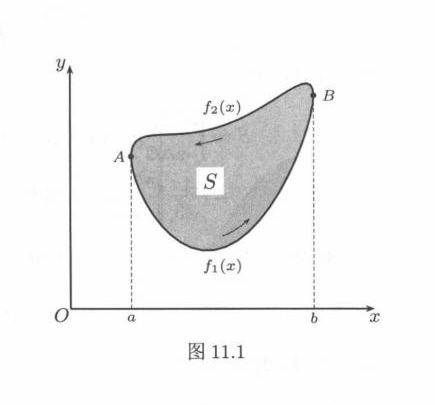
\includegraphics[width=.48\linewidth]{figures/upper/ch11/fig-11-1.png}
\end{center}

这样就可以计算封闭曲线所包含的图形面积如下：
\begin{align*}
S&=\int_a^b[f_2(x)-f_1(x)]\,\dd x\\
 &=\int_\beta^\gamma y(t)\,\dd x(t)-\int_\alpha^\gamma y(t)\,\dd x(t)
 =-\int_\alpha^\beta y(t)\,\dd x(t),
\end{align*}
由分部积分又可得到
\[
  S=-y(t)x(t)\big|_\alpha^\beta+\int_\alpha^\beta x(t)\,\dd y(t)
  =\int_\alpha^\beta x(t)\,\dd y(t).
\]
取两者的平均值就得到公式(11.1)。

\paragraph{注1} 从证明中可见实际上得到了计算面积$S$的三个公式。但是将前两个取平均值后得到的公式(11.1)在计算中一般较为方便，从下面举例就可明白。此外，如前所说，该公式对于一般的没有自交点的参数曲线都是成立的。

\paragraph{注2} 由于极坐标下的$\theta$就可看成为参数，因此完全可以从公式(11.1)推导出极坐标下的扇形面积计算公式(11.2)（留作11.1.4小节的练习题2）。

\begin{xexample}[11.1.1]
求由方程$x^2+xy+y^2=1$所确定的图形面积。
\end{xexample}
\begin{xsolution}
这就是求174页上图6.5所示椭圆的面积。容易想到的一种思路是：先用解析几何中的转轴方法消去交叉项，由此确定椭圆的长、短半轴，最后用简单的定积分计算即可求出椭圆面积。以下是不用转轴的几种积分解法。

\textbf{解1}\quad 从方程解出
\[
  y_{1,2}(x)=-\frac{x}{2}\pm\sqrt{1-\frac34x^2},\qquad
  -\frac{2}{\sqrt3}\le x\le\frac{2}{\sqrt3},
\]
然后计算定积分
\begin{align*}
S&=\int_{-2/\sqrt3}^{2/\sqrt3}[y_1(x)-y_2(x)]\,\dd x
 =2\int_{-2/\sqrt3}^{2/\sqrt3}\sqrt{1-\frac34x^2}\,\dd x\\
 &=\frac4{\sqrt3}\int_{-\pi/2}^{\pi/2}\cos^2\theta\,\dd\theta
 =\frac{2\pi}{\sqrt3}.
\end{align*}

\textbf{解2}\quad 用极坐标，以$x=r\cos\theta,y=r\sin\theta$代入方程，得到
\[
  r^2=\frac1{1+\sin\theta\cos\theta}.
\]
用公式(11.2)计算定积分：
\[
  S=\frac12\int_0^{2\pi}r^2\,\dd\theta
  =\frac12\int_0^{2\pi}\frac{\dd\theta}{1+\frac12\sin2\theta}
  =\int_0^{2\pi}\frac{\dd\varphi}{2+\sin\varphi}
  =\frac{2\pi}{\sqrt3}.
\]
\paragraph{注1} 一个更简单的方法是：从表达式$r^{-2}=1+\frac12\sin2\theta$出发，求出$r$的最大值和最小值，即椭圆的长半轴和短半轴，然后利用椭圆面积公式就可计算出$S$。

\textbf{解3}\quad 先将方程左边配方为
\[
  x^2+xy+y^2=\frac34x^2+\left(y+\frac{x}{2}\right)^2=1,
\]
然后引入参数方程
\[
  x=\frac2{\sqrt3}\cos t,\qquad
  y=\sin t-\frac1{\sqrt3}\cos t,\qquad 0\le t\le2\pi.
\]
由于
\begin{align*}
x(t)y'(t)-y(t)x'(t)
&=\frac2{\sqrt3}\cos t\left(\cos t+\frac1{\sqrt3}\sin t\right)
 -\left(\sin t-\frac1{\sqrt3}\cos t\right)\left(-\frac2{\sqrt3}\sin t\right)\\
&=\frac2{\sqrt3},
\end{align*}
因此最后的定积分计算极其简单：
\[
  S=\frac12\int_0^{2\pi}(x\,\dd y-y\,\dd x)
  =\frac12\int_0^{2\pi}\frac2{\sqrt3}\,\dd t
  =\frac{2\pi}{\sqrt3}.
\]
\paragraph{注2} 在[59]第二册的习题2406的讲解中，列举了求椭圆
\[
  Ax^2+2Bxy+Cy^2=1\qquad(A>0,\Delta=AC-B^2>0)
\]
所围面积的10种解法，其中解8和解9是多元微积分知识的应用，解10则是代数方法。此外，还对于这些解法能否推广做了一点评论。
\end{xsolution}

\begin{xexample}[11.1.2]
求由$y^2-2xy+x^3=0$所确定的封闭曲线所包围的图形面积。
\end{xexample}
\begin{xsolution}
\textbf{分析}\quad 为了知道图形的形状，需要找出$y$随$x$变化的规律。为此需要引入参数。令$y=tx$是常用的方法。这样就可以得到参数方程：
\[
  x=2t-t^2,\qquad y=2t^2-t^3.
\]
首先分析$x=x(t)$和$y=y(t)$的变化情况，然后就不难合成$xOy$坐标平面上的曲线。利用这些分析就可以画出题设的曲线图形如图11.2所示。（参看例题8.6.1中对于类似问题的分析。）当变量$t$从0到2时点$(x(t),y(t))$从原点出发又回到原点，恰好按照逆时针方向描出图中的一条封闭曲线。

\begin{center}
  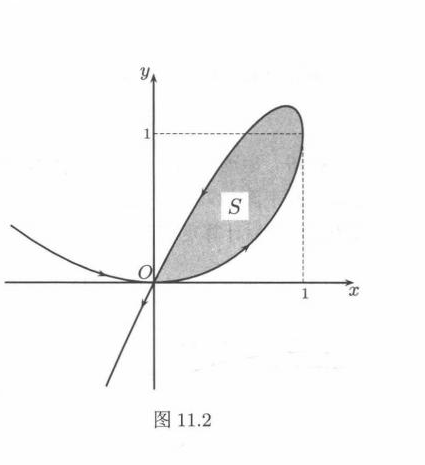
\includegraphics[width=.42\linewidth]{figures/upper/ch11/fig-11-2.png}
\end{center}

\textbf{解1}\quad 利用直角坐标下的公式。由于不难从方程直接解出
\[
  y_{1,2}(x)=x(1\pm\sqrt{1-x}),\qquad 0\le x\le1,
\]
因此就有
\begin{align*}
S&=\int_0^1(x+x\sqrt{1-x})\,\dd x-\int_0^1(x-x\sqrt{1-x})\,\dd x
 =2\int_0^1x\sqrt{1-x}\,\dd x\\
 &=2\int_0^1(1-t)\sqrt t\,\dd t
 =2\left(\frac23t^{3/2}-\frac25t^{5/2}\right)\Big|_0^1
 =\frac8{15}.
\end{align*}

\textbf{解2}\quad 用公式(11.1)：
\begin{align*}
S&=\frac12\int_0^2(x\,\dd y-y\,\dd x)
 =\frac12\int_0^2[(2t-t^2)\,\dd(2t^2-t^3)-(2t^2-t^3)\,\dd(2t-t^2)]\\
 &=\frac12\int_0^2(4t^2-4t^3+t^4)\,\dd t
 =\frac8{15}.
\end{align*}
\end{xsolution}

\begin{xexample}[11.1.3]
设曲线方程为$y=\int_0^x\sqrt{\sin t}\,\dd t,0\le x\le\pi$，求曲线的长度。
\end{xexample}
\begin{xsolution}
记方程为$y=f(x)$，由弧长公式计算定积分：
\begin{align*}
l&=\int_0^\pi\sqrt{1+f'^2(x)}\,\dd x
 =\int_0^\pi\sqrt{1+\sin x}\,\dd x\\
 &=\int_0^\pi\left(\sin\frac x2+\cos\frac x2\right)\,\dd x
 \quad\left(\text{作代换 }t=\frac x2\right)\\
 &=2\left(\int_0^{\pi/2}\sin t\,\dd t+\int_0^{\pi/2}\cos t\,\dd t\right)
 =4\int_0^{\pi/2}\sin t\,\dd t=4.
\end{align*}
\end{xsolution}

\begin{xexample}[11.1.4]
求双曲抛物面$z=x^2-y^2$与平面$x=1,z=0$所围成的立体体积。
\end{xexample}
\begin{xsolution}
\textbf{分析}\quad 如图11.3所示，该立体不是旋转体。我们将用两种方法求解。先计算平行于坐标平面$yOz$的平面或平行于坐标平面$xOy$的平面截立体所得的面积$A(x)$或$B(z)$，然后计算定积分
\[
  \int_0^1A(x)\,\dd x\quad\text{或}\quad\int_0^1B(z)\,\dd z
\]
得到所论立体的体积。

\begin{center}
  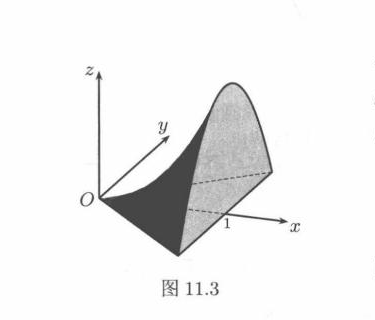
\includegraphics[width=.42\linewidth]{figures/upper/ch11/fig-11-3.png}
\end{center}

\textbf{解1}\quad $x$的变化范围是$0\le x\le1$。对每一个固定的$x\in[0,1]$，计算截面积$A(x)$时，$z=x^2-y^2$成为抛物线的方程，其中$y\in[-x,x]$。从而得到
\[
  A(x)=2\int_0^x(x^2-y^2)\,\dd y
  =2\left(x^3-\frac13x^3\right)=\frac43x^3.
\]
因此，所求的体积为
\[
  V=\frac43\int_0^1x^3\,\dd x=\frac13.
\]

\textbf{解2}\quad $z$的变化范围也是$0\le z\le1$，这可由$x=1$时$z=1-y^2$，而$\abs{y}\le1$得到。计算$B(z)$时，也应把$z$看作在$[0,1]$上取值的固定数，于是$z=x^2-y^2$成为双曲线方程$y^2=x^2-z,x\in[\sqrt z,1]$或$y=\pm\sqrt{x^2-z},x\in[\sqrt z,1]$。这样，$B(z)$便是平面$Z=z$上的上述双曲线与$x=1$围成的弓形面积，因此利用图形关于$x$轴的对称性，可以计算得到
\begin{align*}
B(z)&=2\int_{\sqrt z}^1\sqrt{x^2-z}\,\dd x\\
&=\left(x\sqrt{x^2-z}-z\ln(x+\sqrt{x^2-z})\right)\Big|_{\sqrt z}^1\\
&=\sqrt{1-z}-z\ln(1+\sqrt{1-z})+z\ln\sqrt z.
\end{align*}
因此所求的体积为
\[
  V=\int_0^1B(z)\,\dd z
  =\int_0^1\sqrt{1-z}\,\dd z-\int_0^1z\ln(1+\sqrt{1-z})\,\dd z+\int_0^1z\ln\sqrt z\,\dd z.
\]
显然这三个积分的计算要比解1中的计算复杂得多（细节从略），最后结果为
\[
  V=\frac23-\frac5{24}-\frac18=\frac13.
\]
\paragraph{注} 由此可见，在利用平行的截面面积求体积的问题中，选择合适的截面是十分重要的。请读者考虑，本题如果通过用平行于坐标平面$xOz$的平面去截所论立体，先计算与$y$有关的截面积后再积分的方法求体积，计算过程是否简便？
\end{xsolution}

\subsection{Guldin定理}

质心是一个物理量。Guldin（古尔丁）的第一和第二定理将求旋转体的体积和侧面积转化为求质心，体现了数学问题与物理问题之间的内在联系。

\begin{xproposition}[11.1.1（质心公式）]
设密度均匀的平面图形分布在直线$X=a,X=b$和$Y=c,Y=d$之间，且对任一$x\in[a,b]$和$y\in[c,d]$，直线$X=x$和$Y=y$截图形的线段长度为$s(x)$和$t(y)$，则图形的质心的横坐标与纵坐标分别为
\begin{equation}
  x_c=\frac{\int_a^b xs(x)\,\dd x}{\int_a^b s(x)\,\dd x},\qquad
  y_c=\frac{\int_c^d yt(y)\,\dd y}{\int_c^d t(y)\,\dd y}.
  \tag{11.3}
  \label{eq:11.3}
\end{equation}
而密度均匀的分段光滑曲线$y=f(x)$（$a\le x\le b$）的质心的横坐标与纵坐标分别为
\begin{equation}
  x_c=\frac{\int_a^b x\sqrt{1+f'^2(x)}\,\dd x}{\int_a^b\sqrt{1+f'^2(x)}\,\dd x},\qquad
  y_c=\frac{\int_a^b f(x)\sqrt{1+f'^2(x)}\,\dd x}{\int_a^b\sqrt{1+f'^2(x)}\,\dd x}.
  \tag{11.4}
  \label{eq:11.4}
\end{equation}
\end{xproposition}

由上面的质心公式，可以得到下面两条定理（证明见[59]第二册§4.9）。

\begin{xproposition}[11.1.2（Guldin第一定理）]
设平面曲线的质心坐标为$(x_c,y_c)$，且曲线位于右半平面内，则曲线绕$y$轴旋转一周所产生的旋转曲面的面积$S_y$等于质心绕$y$轴一周所经过的路程$2\pi x_c$乘以曲线的弧长$l$，即$S_y=2\pi x_cl$。
\end{xproposition}

\begin{xproposition}[11.1.3（Guldin第二定理）]
设平面图形的质心坐标为$(x_c,y_c)$，且图形位于右半平面内，则图形绕$y$轴旋转一周所产生的旋转立体的体积$V_y$等于质心绕$y$轴一周所经过的路程$2\pi x_c$乘以图形的面积$S$，即$V_y=2\pi x_cS$。
\end{xproposition}

\begin{xexample}[11.1.5]
设曲线$y=f(x)$（$a\le x\le b$）分段光滑。求曲边梯形
\[
  \{(x,y)\mid 0\le a\le x\le b,\ 0\le y\le f(x)\}
\]
绕$y$轴旋转一周得到的旋转体体积。
\end{xexample}
\begin{xsolution}
\textbf{解1}\quad 由微元法，对曲边梯形在充分小的区间$[x,x+\Delta x]\subseteq[a,b]$上的部分，取$\xi\in[x,x+\Delta x]$。我们用过点$(\xi,f(\xi))$而平行于$x$轴的直线段代替$y=f(x)$的对应曲线段，然后将所得到的矩形绕$y$轴旋转一周，这样得到的旋转体体积为
\[
  \Delta V=\pi f(\xi)[(x+\Delta x)^2-x^2]
  =\pi f(\xi)[2x\Delta x-(\Delta x)^2],
\]
舍弃高阶无穷小量$\pi f(\xi)(\Delta x)^2$后在$[a,b]$上积分，就得到旋转体体积
\[
  V=2\pi\int_a^bxf(x)\,\dd x.
\]

\textbf{解2}\quad 由Guldin第二定理，曲边梯形$\{(x,y)\mid 0\le a\le x\le b,0\le y\le f(x)\}$绕$y$轴旋转一周得到的旋转体体积等于曲边梯形的质心$(x_c,y_c)$绕$y$轴一周所经过的路程$2\pi x_c$乘以图形的面积$S$，即有
\begin{equation}
  V=2\pi x_cS.
  \tag{11.5}
  \label{eq:11.5}
\end{equation}
将质心公式(11.3)中关于$x_c$的公式与曲边梯形的面积公式$S=\int_a^bf$代入(11.5)，便得到
\[
  V=2\pi\frac{\int_a^bxf(x)\,\dd x}{\int_a^bf(x)\,\dd x}\cdot\int_a^bf(x)\,\dd x
  =2\pi\int_a^bxf(x)\,\dd x.
\]
\end{xsolution}

\begin{xexample}[11.1.6]
求上题的旋转体中由曲线$y=f(x)$（$a\le x\le b$）生成的侧面积。
\end{xexample}
\begin{xsolution}
\textbf{解1}\quad 由以曲代直法，曲线$y=f(x)$在充分小的区间$[x,x+\Delta x]\subseteq[a,b]$上的曲线段绕$y$轴旋转一周得到的面积可用连接点$(x,f(x))$与点$(x+\Delta x,f(x+\Delta x))$的直线段绕$y$轴旋转一周得到的圆台的侧面积来代替，即
\begin{align*}
\Delta S_{\text{侧}}
&=2\pi\cdot\frac12[x+(x+\Delta x)]\sqrt{(\Delta x)^2+(\Delta f(x))^2}\\
&=2\pi\cdot\frac12[x+(x+\Delta x)]\sqrt{1+\left(\frac{\Delta f(x)}{\Delta x}\right)^2}\Delta x.
\end{align*}
舍弃高阶无穷小量$\pi\sqrt{1+(\Delta f(x)/\Delta x)^2}(\Delta x)^2$后在$[a,b]$上积分，得旋转体侧面积
\[
  S_{\text{侧}}=2\pi\int_a^bx\sqrt{1+f'^2(x)}\,\dd x.
\]

\textbf{解2}\quad 由Guldin第一定理，所求的侧面积等于曲线段$y=f(x)$（$a\le x\le b$）的质心$(x_c,y_c)$绕$y$轴一周所经过的路程$2\pi x_c$乘以曲线的弧长$l$，即有
\begin{equation}
  S_{\text{侧}}=2\pi x_cl.
  \tag{11.6}
  \label{eq:11.6}
\end{equation}
将弧长公式$l=\int_a^b\sqrt{1+(f'(x))^2}\,\dd x$与质心公式(11.4)中$x_c$的公式代入(11.6)，便得到
\[
  S_{\text{侧}}=2\pi\int_a^bx\sqrt{1+f'^2(x)}\,\dd x.
\]
\end{xsolution}

\subsection{练习题}

由于在习题集[27]（及其学习指引[59]）和各种教科书中都有许多几何计算题可用，因此本节只收入少量练习题作为补充。

\begin{xexercise}[1]
设椭圆方程为$Ax^2+2Bxy+Cy^2=1$，其中$A>0,\Delta=AC-B^2>0$。试用例题11.1.1中的第三种方法（即公式(11.1)）证明：由该椭圆所围的面积等于$\pi/\sqrt\Delta$。
\end{xexercise}
\begin{xsolution}
由$A>0$及$\Delta=AC-B^2>0$知$C>0$。将二次型配方：
\[
 Ax^2+2Bxy+Cy^2
 =C\left(y+\frac BCx\right)^2+\frac{\Delta}{C}x^2.
\]
因此椭圆可参数化为
\[
 x=\sqrt{\frac C\Delta}\cos t,\qquad
 y=\frac1{\sqrt C}\sin t-\frac{B}{\sqrt{C\Delta}}\cos t,\qquad 0\le t\le2\pi.
\]
由
\[
 x'(t)=-\sqrt{\frac C\Delta}\sin t,
 \qquad
 y'(t)=\frac1{\sqrt C}\cos t+
 \frac{B}{\sqrt{C\Delta}}\sin t,
\]
可得
\begin{align*}
x(t)y'(t)-y(t)x'(t)
&=\frac1{\sqrt\Delta}(\cos^2t+\sin^2t)\\
&=\frac1{\sqrt\Delta}.
\end{align*}
由公式(11.1)，
\[
 S=\frac12\int_0^{2\pi}\bigl(xy'-yx'\bigr)\,\dd t
 =\frac12\int_0^{2\pi}\frac{\dd t}{\sqrt\Delta}
 =\frac\pi{\sqrt\Delta}.
\]
\end{xsolution}


\begin{xexercise}[2]
试以公式(11.1)为出发点，推导出极坐标下的扇形面积计算公式(11.2)。
\end{xexercise}
\begin{xsolution}
在极坐标中写
\[
 x=\rho(\theta)\cos\theta,\qquad
 y=\rho(\theta)\sin\theta.
\]
于是
\begin{align*}
\dd x&=(\rho'\cos\theta-\rho\sin\theta)\,\dd\theta,\\
\dd y&=(\rho'\sin\theta+\rho\cos\theta)\,\dd\theta,
\end{align*}
从而沿曲线$\rho=\rho(\theta)$有
\[
 x\,\dd y-y\,\dd x
 =\rho^2(\theta)\,\dd\theta.
\]
扇形边界还包括$\theta=\theta_1,\theta_2$上的两条径向线段。固定其中一个极角$\theta_i$，以$r$为参数写成$x=r\cos\theta_i,y=r\sin\theta_i$，则
\[
 x\,\dd y-y\,\dd x
 =r\cos\theta_i\sin\theta_i\,\dd r-r\sin\theta_i\cos\theta_i\,\dd r=0.
\]
所以把整个封闭边界代入(11.1)，只有曲线$\rho=\rho(\theta)$这一段有贡献，得到
\[
 S=\frac12\int_{\theta_1}^{\theta_2}\rho^2(\theta)\,\dd\theta,
\]
即公式(11.2)。
\end{xsolution}


\begin{xexercise}[3]
已知三个半径为$r$的圆，其中每个圆的圆周都通过另外两个圆的圆心，求三个圆公共部分的面积。

  （本题有不用微积分的初等解法。）
\end{xexercise}
\begin{xsolution}
三个圆心两两距离均为$r$，故三个圆心组成边长为$r$的正三角形。三个圆的公共部分是Reuleaux三角形。每一个边界圆弧所对的圆心角均为$\pi/3$。

公共部分可看成三个半径为$r$、圆心角为$\pi/3$的扇形之和，再减去两个正三角形的面积。因此
\[
 S=3\cdot\frac12r^2\frac\pi3
 -2\cdot\frac{\sqrt3}{4}r^2
 =\frac{\pi-\sqrt3}{2}r^2.
\]
\end{xsolution}


\begin{xexercise}[4]
周长一定的等腰三角形，腰与底的比例为多少时，它绕底边旋转所得的旋转体体积最大？
\end{xexercise}
\begin{xsolution}
设等腰三角形的腰长为$l$，底边长为$b$，周长为$P$，则
\[
 2l+b=P.
\]
三角形绕底边旋转所得立体由两个同底圆锥组成。若三角形的高为$h$，则
\[
 h^2=l^2-\frac{b^2}{4},
\]
总的体积为
\[
 V=\frac13\pi h^2b
 =\frac\pi3b\left(l^2-\frac{b^2}{4}\right).
\]
由$l=(P-b)/2$，
\[
 V=\frac\pi{12}b(P^2-2Pb),\qquad 0<b<\frac P2.
\]
故
\[
 V'(b)=\frac\pi{12}(P^2-4Pb).
\]
唯一的内点极大值在$b=P/4$处取得，此时$l=3P/8$。因此
\[
 \boxed{\frac lb=\frac32}.
\]
\end{xsolution}


\begin{xexercise}[5]
半轴长为$a$和$b$的一个椭圆在曲线$y=c\sin(x/a)$上进行无滑动的滚动。问$a,b,c$之间的关系怎样时，椭圆在曲线上滚动了曲线的一个周期时，它正好转了一周？
\end{xexercise}
\begin{xsolution}
曲线$y=c\sin(x/a)$的一个周期在$x$方向的长度为$2\pi a$，其弧长为
\begin{align*}
L&=\int_0^{2\pi a}\sqrt{1+\frac{c^2}{a^2}\cos^2\frac xa}\,\dd x\\
&=\int_0^{2\pi}\sqrt{a^2+c^2\cos^2 t}\,\dd t\\
&=\int_0^{2\pi}\sqrt{a^2\sin^2 t+(a^2+c^2)\cos^2 t}\,\dd t.
\end{align*}
无滑动滚动一周时，接触曲线走过的弧长必须等于椭圆周长。椭圆半轴为$a,b$时周长为
\[
 P=\int_0^{2\pi}\sqrt{a^2\sin^2 t+b^2\cos^2 t}\,\dd t.
\]
在$b>0$时，该积分关于$b$严格增加，因此$L=P$当且仅当
\[
 b^2=a^2+c^2.
\]
故所求关系为
\[
 \boxed{b^2=a^2+c^2}.
\]
\end{xsolution}


\begin{xexercise}[6]
在单位圆周上任意取一段位于第一象限且长度为$s$的弧，设位于该弧下方、$x$轴上方的曲边梯形的面积为$A$，而位于该弧左侧、$y$轴右侧的曲边梯形的面积为$B$。证明：$A+B$只依赖于弧的长度$s$，而与弧的位置无关。
\end{xexercise}
\begin{xsolution}
设该弧的两个端点所对应的极角为$\alpha<\beta$。单位圆上弧长等于圆心角，故
\[
 s=\beta-\alpha.
\]
沿弧取参数$x=\cos\theta,y=\sin\theta$，$\alpha\le\theta\le\beta$。弧下方、$x$轴上方的面积为
\[
 A=-\int_{\alpha}^{\beta}y\,\dd x
 =\int_\alpha^\beta\sin^2\theta\,\dd\theta,
\]
弧左侧、$y$轴右侧的面积为
\[
 B=\int_{\alpha}^{\beta}x\,\dd y
 =\int_\alpha^\beta\cos^2\theta\,\dd\theta.
\]
因此
\[
 A+B=\int_\alpha^\beta(\sin^2\theta+\cos^2\theta)\,\dd\theta
 =\beta-\alpha=s.
\]
所以$A+B$只依赖于弧长$s$，与弧在第一象限中的位置无关。
\end{xsolution}


\begin{xexercise}[7]
试求由抛物线$y^2=2x$与过其焦点的弦所围的图形面积的最小值。
\end{xexercise}
\begin{xsolution}
抛物线$y^2=2x$可参数化为
\[
 x=\frac{t^2}{2},\qquad y=t.
\]
设过焦点$(1/2,0)$的弦的两个端点参数为$t_1<t_2$。两参数点的弦方程为
\[
 x=\frac{t_1+t_2}{2}y-\frac{t_1t_2}{2}.
\]
该弦通过焦点的充要条件是$t_1t_2=-1$。

用$y$作积分变量，弦与抛物线之间的面积为
\begin{align*}
S&=\int_{t_1}^{t_2}\left[
\frac{t_1+t_2}{2}y-\frac{t_1t_2}{2}-\frac{y^2}{2}
\right]\,\dd y\\
&=\frac12\int_{t_1}^{t_2}(y-t_1)(t_2-y)\,\dd y
=\frac{(t_2-t_1)^3}{12}.
\end{align*}
令$t_2=t>0,t_1=-1/t$，则
\[
 t_2-t_1=t+\frac1t\ge2.
\]
故
\[
 S\ge\frac{2^3}{12}=\frac23.
\]
等号在$t=1$时取得，即弦为通径$x=1/2$。所以最小面积为
\[
 \boxed{\frac23}.
\]
\end{xsolution}


\begin{xexercise}[8]
至少用两种方法计算下列三个圆的公共部分的面积：
  \[
    x^2+y^2\le4,\qquad (x-2)^2+y^2\le4,\qquad x^2+(y-2)^2\le4.
  \]
\end{xexercise}
\begin{xsolution}
记公共部分为$D$。

\textbf{方法一（极坐标）}\quad 三个圆盘的条件分别为
\[
 r\le2,\qquad r\le4\cos\theta,\qquad r\le4\sin\theta,
\]
且$0\le\theta\le\pi/2$。因此
\[
 r_{\max}(\theta)=
 \begin{cases}
 4\sin\theta,&0\le\theta\le\pi/6,\\
 2,&\pi/6\le\theta\le\pi/3,\\
 4\cos\theta,&\pi/3\le\theta\le\pi/2.
 \end{cases}
\]
于是
\begin{align*}
|D|
&=\frac12\left[
\int_0^{\pi/6}16\sin^2\theta\,\dd\theta
+\int_{\pi/6}^{\pi/3}4\,\dd\theta
+\int_{\pi/3}^{\pi/2}16\cos^2\theta\,\dd\theta
\right]\\
&=16\int_0^{\pi/6}\sin^2\theta\,\dd\theta+\frac\pi3\\
&=\frac{5\pi}{3}-2\sqrt3.
\end{align*}

\textbf{方法二（直角坐标）}\quad 对固定$x$，公共部分的下边界为
\[
 y=2-\sqrt{4-x^2}.
\]
当$0\le x\le1$时，上边界来自圆$(x-2)^2+y^2=4$；当$1\le x\le\sqrt3$时，上边界来自圆$x^2+y^2=4$。所以
\begin{align*}
|D|
&=\int_0^1\left[\sqrt{4-(x-2)^2}-2+\sqrt{4-x^2}\right]\,\dd x\\
&\quad+\int_1^{\sqrt3}\left[2\sqrt{4-x^2}-2\right]\,\dd x.
\end{align*}
利用
\[
 \int\sqrt{4-x^2}\,\dd x
 =\frac x2\sqrt{4-x^2}+2\arcsin\frac x2
\]
逐项代入端点，整理同样得到
\[
 |D|=\boxed{\frac{5\pi}{3}-2\sqrt3}.
\]
\end{xsolution}


\begin{xexercise}[9]
求椭圆柱$x^2/16+y^2/100\le1$夹在平面$z=0,y=2z$之间部分的体积。
\end{xexercise}
\begin{xsolution}
平面$y=2z$写成$z=y/2$。在椭圆柱的每一个竖直截线上，两平面$z=0$与$z=y/2$之间的高度为$\abs{y}/2$。故体积
\[
 V=\frac12\iint_D\abs{y}\,\dd x\,\dd y,
 \qquad
 D:\ \frac{x^2}{16}+\frac{y^2}{100}\le1.
\]
利用关于$x$轴的对称性，
\begin{align*}
V&=\iint_{D\cap\{y\ge0\}}y\,\dd x\,\dd y\\
&=\int_0^{10}8y\sqrt{1-\frac{y^2}{100}}\,\dd y
=\frac{800}{3}.
\end{align*}
因此
\[
 \boxed{V=\frac{800}{3}}.
\]
\end{xsolution}


\begin{xexercise}[10]
求圆柱面$x^2+y^2=a^2$与$x^2+z^2=a^2$所围立体区域的体积。

  （这个立体区域在中国古代数学史上称为牟合方盖，它是刘徽在研究球体积计算问题中提出来的，见[35]。在这之前，Archimedes在其著作《方法》的命题15中已经给出了这个立体区域的体积计算（参见[60]的192页）。）
\end{xexercise}
\begin{xsolution}
立体区域满足
\[
 x^2+y^2\le a^2,\qquad x^2+z^2\le a^2.
\]
固定$x\in[-a,a]$后，$y,z$都在区间
\[
 -\sqrt{a^2-x^2}\le y,z\le\sqrt{a^2-x^2}
\]
内，因此垂直于$x$轴的截面是边长$2\sqrt{a^2-x^2}$的正方形，面积
\[
 A(x)=4(a^2-x^2).
\]
故
\[
 V=\int_{-a}^a4(a^2-x^2)\,\dd x
 =\boxed{\frac{16}{3}a^3}.
\]
\end{xsolution}


\section{不等式}

在§1.3和§8.5已经接触到了许多不等式。现在有了积分学的工具，可以得到的不等式就更多了。由于这方面的材料较多，我们将分成几小节来介绍。

\subsection{凸函数不等式}

凸函数的基本定义和主要理论见§8.4和第八章的部分参考题。需要指出，本书中的下凸函数和上凸函数分别与有的文献中的凸函数和凹函数相对应。

在含有积分的凸函数不等式中，先介绍Hadamard不等式。

\begin{xexample}[11.2.1（Hadamard不等式）]
设$f$是$(a,b)$上的下凸函数，则对每一对$x_1,x_2\in(a,b),x_1<x_2$，有
\begin{equation}
  f\left(\frac{x_1+x_2}{2}\right)
  \le\frac1{x_2-x_1}\int_{x_1}^{x_2}f(t)\,\dd t
  \le\frac{f(x_1)+f(x_2)}2.
  \tag{11.7}
  \label{eq:11.7}
\end{equation}
\end{xexample}

从图11.4上可以看出Hadamard不等式具有明显的几何意义。由于$f$是$[a,b]$上的下凸函数，曲线段$y=f(x)$（$x_1\le x\le x_2$）位于曲线过点$\left(\frac12(x_1+x_2),f\left(\frac12(x_1+x_2)\right)\right)$的切线段上方\footnote{见命题8.4.5。若$f$于该点不可导，则用8.4.2小节的题11中的支撑线代替切线。}，并位于连接点$(x_1,f(x_1))$与点$(x_2,f(x_2))$的直线段下方，因此曲线段$y=f(x)$（$x_1\le x\le x_2$）与直线$x=x_1,x=x_2$及$x$轴围成的曲边梯形面积应在上述两直线段分别与直线$x=x_1,x=x_2$及$x$轴围成的两个梯形的面积之间。

\begin{center}
  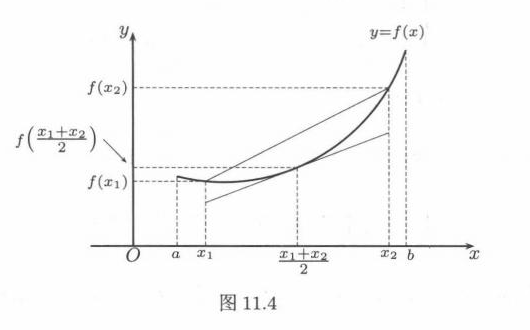
\includegraphics[width=.56\linewidth]{figures/upper/ch11/fig-11-4.png}
\end{center}

\begin{xproof}
从命题8.4.2知道$f$连续，因此可积性没有问题。注意到点$\frac12(x_1+x_2)$不仅是$x_1$和$x_2$的中点，同时也是$x_1+\lambda(x_2-x_1)$和$x_2-\lambda(x_2-x_1)$的中点，其中$\lambda\in[0,1]$。利用$f$为下凸函数，则就有不等式
\begin{equation}
  \frac12[f(x_1+\lambda(x_2-x_1))+f(x_2-\lambda(x_2-x_1))]
  \ge f\left(\frac{x_1+x_2}{2}\right).
  \tag{11.8}
  \label{eq:11.8}
\end{equation}
将上式两边对$\lambda$从0到1积分，经计算后就可以得到
\begin{equation}
  \frac1{x_2-x_1}\int_{x_1}^{x_2}f(t)\,\dd t
  \ge f\left(\frac{x_1+x_2}{2}\right).
  \tag{11.9}
  \label{eq:11.9}
\end{equation}
另一方面，由$f$是下凸函数又可得到
\begin{align*}
\frac1{x_2-x_1}\int_{x_1}^{x_2}f(t)\,\dd t
&=\int_0^1f(\lambda x_2+(1-\lambda)x_1)\,\dd\lambda\\
&\le\int_0^1[\lambda f(x_2)+(1-\lambda)f(x_1)]\,\dd\lambda\\
&=\frac{f(x_1)+f(x_2)}2.
\end{align*}
\end{xproof}

\paragraph{注} Hadamard不等式(11.7)含有左边和右边的两个不等式。可以证明，其中每一个不等式都是函数下凸的充分必要条件。还可以证明，若其中任何一个不等式对所有$x_1,x_2\in(a,b)$成立等号，则$f$只能是线性函数（留作本章第二组参考题7）。

第二个重要的凸函数不等式可以从命题8.4.7（Jensen不等式）取极限得到：

\begin{xproposition}[11.2.1（Jensen不等式）]
设$f,p\in R[a,b],m\le f(x)\le M,p(x)$非负且$\int_a^bp(x)\,\dd x>0$，则当$\varphi$是$[m,M]$上的下凸函数时，成立不等式：
\[
  \varphi\left(\frac{\int_a^bp(x)f(x)\,\dd x}{\int_a^bp(x)\,\dd x}\right)
  \le\frac{\int_a^bp(x)\varphi(f(x))\,\dd x}{\int_a^bp(x)\,\dd x}.
\]
若$\varphi$为上凸函数则不等式反向。
\end{xproposition}

Jensen不等式包含了很多不等式。取$p(x)=1$，就得到
\[
  \varphi\left(\frac1{b-a}\int_a^bf(t)\,\dd t\right)
  \le\frac1{b-a}\int_a^b\varphi(f(t))\,\dd t.
\]
又若$\int_a^bp(x)\,\dd x=1$，并利用$\ee^x$为下凸函数和$\ln x$为上凸函数就得到
\begin{equation}
  \exp\left(\int_a^bp(x)\ln f(x)\,\dd x\right)
  \le\int_a^bp(x)f(x)\,\dd x
  \le\ln\left(\int_a^bp(x)\exp f(x)\,\dd x\right).
  \tag{11.10}
  \label{eq:11.10}
\end{equation}
左边的不等式就是广义的平均值不等式（命题8.5.1）的积分形式。

下一个不等式也是Jensen不等式的特例。设$f\in R[a,b],f(x)\ge m>0$，则成立不等式：
\[
  \ln\left(\frac1{b-a}\int_a^bf(x)\,\dd x\right)
  \ge\frac1{b-a}\int_a^b\ln f(x)\,\dd x.
\]
以上的每个不等式又包含了许多具体的不等式。例如

\begin{xexample}[11.2.2]
若$f$为$[0,1]$上的上凸函数，则对每个正整数$n$成立不等式：
\[
  \int_0^1f(x^n)\,\dd x\le f\left(\frac1{n+1}\right).
\]
\end{xexample}

\subsection{Schwarz积分不等式}

Schwarz积分不等式是最基本的积分不等式之一，应用非常广泛。

\begin{xproposition}[11.2.2（Schwarz积分不等式）]
设$f,g\in R[a,b]$，则
\[
  \left(\int_a^bf(x)g(x)\,\dd x\right)^2
  \le\int_a^bf^2(x)\,\dd x\int_a^bg^2(x)\,\dd x.
\]
\end{xproposition}

\begin{xproof}
\textbf{证1}\quad （用证明Cauchy不等式（命题1.3.5）的同样方法。）如果$\int_a^bf^2(x)\,\dd x$与$\int_a^bg^2(x)\,\dd x$两个积分中至少有一个不等于0，我们不妨设$\int_a^bf^2(x)\,\dd x\ne0$。由于对一切实数$\lambda$，在$[a,b]$上$[\lambda f(x)-g(x)]^2\ge0$，因此有
\[
  \int_a^b[\lambda f(x)-g(x)]^2\,\dd x\ge0.
\]
将它展开，得到关于$\lambda$的非负二次三项式
\[
  \lambda^2\int_a^bf(x)^2\,\dd x-2\lambda\int_a^bf(x)g(x)\,\dd x+\int_a^bg^2(x)\,\dd x\ge0,
\]
因此它的判别式$\Delta\le0$，即
\[
  \left(\int_a^bf(x)g(x)\,\dd x\right)^2
  -\int_a^bf^2(x)\,\dd x\int_a^bg^2(x)\,\dd x\le0,
\]
移项即得所欲证的不等式。

如果积分$\int_a^bf^2(x)\,\dd x=\int_a^bg^2(x)\,\dd x=0$，则可以如下证明：
\begin{align*}
\abs{\int_a^bf(x)g(x)\,\dd x}
&\le\int_a^b\abs{f(x)g(x)}\,\dd x\\
&\le\int_a^b\frac{f^2(x)+g^2(x)}2\,\dd x\\
&=\frac12\int_a^bf^2(x)\,\dd x+\frac12\int_a^bg^2(x)\,\dd x=0.
\end{align*}

\textbf{证2}\quad 将$[a,b]$作等距分划，令$x_i=a+\frac in(b-a),i=0,1,\ldots,n$，应用Cauchy不等式（命题1.3.5）得到
\[
  \left(\frac1n\sum_{i=1}^nf(x_i)g(x_i)\right)^2
  \le\frac1n\sum_{i=1}^nf^2(x_i)\cdot\frac1n\sum_{i=1}^ng^2(x_i),
\]
令$n\to\infty$，即得
\[
  \left(\int_a^bf(x)g(x)\,\dd x\right)^2
  \le\int_a^bf^2(x)\,\dd x\int_a^bg^2(x)\,\dd x.
\]
\end{xproof}

\paragraph{注1} 以上两个证明表明，为了得到与离散不等式对应的积分不等式，经常有两条思路可用：(1)用过去的方法；(2)从对应的离散不等式取极限。

\paragraph{注2} 从证1就可以得到Schwarz不等式成立等号的充分必要条件。实际上，从判别式$\Delta=0$知道存在某个$\lambda_0$，使得$(\lambda_0f-g)^2$在$[a,b]$上的积分等于0。利用第十章的Lebesgue定理（命题10.1.6）和该章的第一组参考题9，可见在$[a,b]$上几乎处处成立$\lambda_0f(x)=g(x)$。回顾证1，这是在$f^2$于区间$[a,b]$上的积分大于0的前提下得到的。对于$g^2$的积分不等于0的情况有类似的结论。

\paragraph{注3} 从上述证明可见Schwarz不等式与Cauchy不等式本质上是同一不等式，只是前者用积分形式表示而已。因此Schwarz不等式也称为Cauchy-Schwarz不等式，或者Cauchy-Schwarz-Bunyakowskii（布尼亚科夫斯基）不等式。

Schwarz积分不等式在本书中有多次应用，下面先举一个例子。

\begin{xexample}[11.2.3]
设$f\in C^1[a,b]$，且$f(a)=0$，证明：
\[
  \int_a^bf^2(x)\,\dd x\le\frac{(b-a)^2}{2}\int_a^b(f'(x))^2\,\dd x.
\]
\end{xexample}
\begin{xproof}
利用条件$f(a)=0$可以写出
\[
  f(x)=\int_a^xf'(t)\,\dd t,
\]
然后用Schwarz不等式作如下估计：
\[
  f^2(x)=\left(\int_a^xf'(t)\,\dd t\right)^2
  \le\left(\int_a^x(f'(t))^2\,\dd t\right)(x-a)
  \le(x-a)\int_a^b(f'(t))^2\,\dd t,
\]
再将两边对$x$从$a$到$b$积分就得到所求的结果。
\end{xproof}

\subsection{其他著名积分不等式}

除了Schwarz不等式，还有许多其他的著名积分不等式。下面我们再介绍三个在分析中的基本不等式，即Young不等式、Hölder积分不等式与Minkowski积分不等式。

\begin{xproposition}[11.2.3（Young不等式）]
设$f$在$[0,+\infty)$上连续可导且严格单调增加，$f(0)=0,a,b>0$，则有
\begin{equation}
  ab\le\int_0^af(x)\,\dd x+\int_0^bg(y)\,\dd y.
  \tag{11.11}
  \label{eq:11.11}
\end{equation}
其中$g(y)$是$f(x)$的反函数，而等号当且仅当$b=f(a)$时成立。
\end{xproposition}

\paragraph{注} Young不等式的几何意义十分清楚。由于定积分在几何上等于曲边梯形的面积，可能发生的只有图11.5所示的(a)、(b)、(c)三种情况。定积分$\int_0^af(x)\,\dd x$和定积分$\int_0^bg(y)\,\dd y$的值在每一张分图中分别等于带有阴影的两个曲边三角形的面积。对于前两种情况，这两个面积之和都严格大于边长为$a$和$b$的矩形面积，而在第三种情况则相等。这个矩形在图11.5(a)和(b)中的边界是由曲边三角形的部分边界和一段虚线构成的。

\begin{center}
  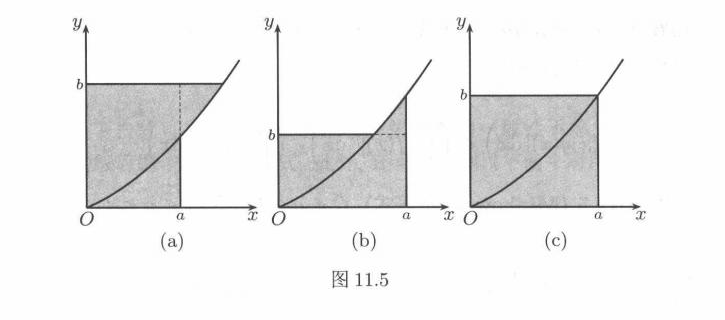
\includegraphics[width=.72\linewidth]{figures/upper/ch11/fig-11-5.png}
\end{center}

\begin{xproof}
将(11.11)右边的两个积分之和记为$I$。利用$g(f(x))\equiv x$，对其中第二个积分作变量代换$y=f(x)$，即$x=g(y)$，然后分部积分得到：
\begin{align}
I&=\int_0^af(x)\,\dd x+\int_0^bg(y)\,\dd y
 =\int_0^af(x)\,\dd x+\int_0^{g(b)}x\,\dd f(x)\notag\\
 &=\int_0^af(x)\,\dd x+xf(x)\big|_0^{g(b)}-\int_0^{g(b)}f(x)\,\dd x\notag\\
 &=bg(b)-\int_a^{g(b)}f(x)\,\dd x.
 \tag{11.12}
 \label{eq:11.12}
\end{align}
其中利用了$f(g(b))=b$。如果$a=g(b)$，也就是$b=f(a)$，则已经得到(11.11)中成立等号的情况（见图11.5(c)）。

在$a<g(b)$时，对于(11.12)中的积分利用$f(x)$在区间$[a,g(b)]$上严格单调增加，$f(x)\le f(g(b))=b$，就得到$I>bg(b)-[g(b)-a]b=ab$。在$a>g(b)$时，类似地可得到
\[
  I=bg(b)+\int_{g(b)}^af(x)\,\dd x>bg(b)+[a-g(b)]b=ab.
\]
\end{xproof}

\paragraph{注} 可以发现以上证明的每一步都有明显的几何意义。此外，Young不等式中的条件“$f\in C^1[0,\infty)$”可以降低为“$f\in C[0,\infty)$”。但这样改变条件后，不能再用分部积分法，而需要从积分定义出发来建立(11.12)。这个证明及Young不等式的另一边估计留作为本章的第二组参考题6。

下面的Hölder不等式和Minkowski不等式都可以从§8.5中对应的离散不等式取极限或者用与那里类似的方法得到，因此这里不再给出证明。

\begin{xproposition}[11.2.4（Hölder不等式）]
设$f,g\in R[a,b]$，$p,q$为满足$1/p+1/q=1$的一对正实数（共轭实数），则成立
\begin{equation}
  \int_a^b\abs{f(x)g(x)}\,\dd x
  \le\left(\int_a^b\abs{f(x)}^p\,\dd x\right)^{1/p}
  \left(\int_a^b\abs{g(x)}^q\,\dd x\right)^{1/q}.
  \tag{11.13}
  \label{eq:11.13}
\end{equation}
\end{xproposition}

\begin{xproposition}[11.2.5（Minkowski不等式）]
设$f,g\in R[a,b]$，$1\le p<+\infty$，则成立
\begin{equation}
  \left(\int_a^b\abs{f(x)+g(x)}^p\,\dd x\right)^{1/p}
  \le\left(\int_a^b\abs{f(x)}^p\,\dd x\right)^{1/p}
  +\left(\int_a^b\abs{g(x)}^p\,\dd x\right)^{1/p}.
  \tag{11.14}
  \label{eq:11.14}
\end{equation}
当$0<p<1$时不等式反向成立。
\end{xproposition}

\paragraph{注} Hölder积分不等式与Minkowski积分不等式是“实变函数”与“泛函分析”课程中的两个基本不等式。当然在那里对于函数$f,g$的条件要更为一般。此外，在Hölder不等式中成立等号的条件是存在常数$c$，使得$\abs{f(x)}^p=c\abs{g(x)}^q$（或者对换$f$和$g$并将$p$换为$q$）；在Minkowski不等式中成立等号的条件是存在非负常数$c$，使得$f(x)=cg(x)$（或者对换$f$和$g$）。但即使是在Riemann可积条件下，这两个条件中的等式都应当理解为几乎处处成立（参见命题10.1.6）。

\subsection{不等式的其他例题}

用积分学方法可以建立过去要用Taylor定理才能得到的某些不等式。下面就是一个例子（见《美国数学月刊》(1990)第97卷912--915页）。

\begin{xexample}[11.2.4]
用积分学方法求出$\sin x$和$\cos x$的一些基本不等式。
\end{xexample}
\begin{xsolution}
在$x>0$时从$\cos x\le1$出发，从0到$x$积分，得到不等式（命题1.3.6）
\[
  \sin x<x.
\]
再对两边从0到$x$积分，得到$1-\cos x<x^2/2$，将它改写为
\[
  \cos x>1-\frac{x^2}{2},
\]
然后再做一次积分得到
\[
  \sin x>x-\frac{x^3}{6},
\]
即例题8.5.3中的不等式。于是已经有
\[
  x-\frac{x^3}{6}<\sin x<x.
\]
再一次积分后可以得到
\[
  1-\frac{x^2}{2}<\cos x<1-\frac{x^2}{2}+\frac{x^4}{24}.
\]
归纳地进行下去就可以得到关于正弦和余弦函数的一般性不等式，其中包括了8.5.3小节的练习题15中的不等式。此外，还可以得到以下两个对所有$x$成立的绝对值不等式
\[
  \abs{\sin x-\sum_{k=0}^n(-1)^k\frac{x^{2k+1}}{(2k+1)!}}
  \le\frac{\abs{x}^{2n+3}}{(2n+3)!},
\]
\[
  \abs{\cos x-\sum_{k=0}^n(-1)^k\frac{x^{2k}}{(2k)!}}
  \le\frac{\abs{x}^{2n+2}}{(2n+2)!}.
\]
此外，对于每个固定的$x$，令$n\to\infty$，就可得到正弦和余弦函数的Taylor级数展开式（参见下册§14.4关于Taylor级数的一般性讨论）。
\end{xsolution}

\begin{xexample}[11.2.5]
设函数$f\in C[a,b]$且单调增加，证明：
\[
  \int_a^bxf(x)\,\dd x\ge\frac{a+b}{2}\int_a^bf(x)\,\dd x.
\]
\end{xexample}
\paragraph{注} 当$f$非负时，本题有明显的物理意义：如果曲线$y=f(x)$单调增加，则密度均匀的曲边梯形
\[
  \{(x,y)\mid a\le x\le b,\ 0\le y\le f(x)\}
\]
的质心不可能落在直线$x=(a+b)/2$的左边（参见(11.3)中关于$x_c$的公式）。

\paragraph{分析} 本题的解法很多（参见[13,30]），下面举出其中的两个证明。关键是要利用$f$的单调性和$x-(a+b)/2$关于积分区间的中点为奇函数的性质。

\begin{xproof}
\textbf{证1}\quad 因为$f$单调增加，所以成立
\begin{equation}
  \left(x-\frac{a+b}{2}\right)\left[f(x)-f\left(\frac{a+b}{2}\right)\right]\ge0.
  \tag{11.15}
  \label{eq:11.15}
\end{equation}
将上式对$x$从$a$到$b$积分，又利用
\[
  \int_a^b\left(x-\frac{a+b}{2}\right)\,\dd x=0,
\]
就可以得到所要的不等式。

\textbf{证2}\quad 将$[a,b]$分为两个区间，分别用第一中值定理，就得到
\begin{align*}
\int_a^b\left(x-\frac{a+b}{2}\right)f(x)\,\dd x
&=\int_a^{(a+b)/2}\left(x-\frac{a+b}{2}\right)f(x)\,\dd x
 +\int_{(a+b)/2}^b\left(x-\frac{a+b}{2}\right)f(x)\,\dd x\\
&=f(\xi_1)\int_a^{(a+b)/2}\left(x-\frac{a+b}{2}\right)\,\dd x
 +f(\xi_2)\int_{(a+b)/2}^b\left(x-\frac{a+b}{2}\right)\,\dd x\\
&=[f(\xi_2)-f(\xi_1)]\cdot\frac{(b-a)^2}{8}\ge0,
\end{align*}
因为其中$a<\xi_1<\frac12(a+b)<\xi_2<b$，而$f$单调增加。
\end{xproof}

下面是对于广义算术平均值—几何平均值不等式（例题8.5.1）的一个新的积分学证明，见《美国数学月刊》(1996)第103卷585页。

\begin{xexample}[11.2.6]
设有$n$个非负数$x_1,\ldots,x_n$和$n$个正数$\lambda_1,\ldots,\lambda_n$，且$\lambda_1+\cdots+\lambda_n=1$，则成立不等式
\begin{equation}
  G_n=\prod_{i=1}^nx_i^{\lambda_i}\le\sum_{i=1}^n\lambda_ix_i=A_n,
  \tag{11.16}
  \label{eq:11.16}
\end{equation}
其中当且仅当$x_1=x_2=\cdots=x_n$时成立等号。
\end{xexample}
\begin{xproof}
只需对$n$个正数$x_1,\ldots,x_n$证明即可。不妨设已有$x_1\le\cdots\le x_n$，则存在$k\in\{1,\ldots,n-1\}$，使得$x_k\le G_n\le x_{k+1}$。这时用拟合法得到
\begin{align*}
\frac{A_n}{G_n}-1
&=\sum_{i=1}^n\lambda_i\left(\frac{x_i-G_n}{G_n}\right)
 =\sum_{i=1}^n\lambda_i\int_{G_n}^{x_i}\frac{\dd t}{G_n}\\
&=-\sum_{i=1}^k\lambda_i\int_{x_i}^{G_n}\frac{\dd t}{G_n}
 +\sum_{i=k+1}^n\lambda_i\int_{G_n}^{x_i}\frac{\dd t}{G_n}.
\end{align*}
又用拟合法（“无中生有”）写出
\begin{align*}
0=\ln G_n-\sum_{i=1}^n\lambda_i\ln x_i
&=\sum_{i=1}^n\lambda_i(\ln G_n-\ln x_i)
 =\sum_{i=1}^n\lambda_i\int_{x_i}^{G_n}\frac{\dd t}{t}\\
&=\sum_{i=1}^k\lambda_i\int_{x_i}^{G_n}\frac{\dd t}{t}
 -\sum_{i=k+1}^n\lambda_i\int_{G_n}^{x_i}\frac{\dd t}{t}.
\end{align*}
将两式相加得到
\[
  \frac{A_n}{G_n}-1
  =\sum_{i=1}^k\lambda_i\int_{x_i}^{G_n}\left(\frac1t-\frac1{G_n}\right)\,\dd t
  +\sum_{i=k+1}^n\lambda_i\int_{G_n}^{x_i}\left(\frac1{G_n}-\frac1t\right)\,\dd t,
\]
由于右边的每一项都非负，因此就得到$A_n\ge G_n$，而且可直接看出等号成立的充分必要条件是$x_i=G_n,i=1,\ldots,n$，也就是$x_1=\cdots=x_n$。
\end{xproof}

\paragraph{注} 这个证明确有新意，但关键并不在于用积分工具。如果对于中间一步的$\ln G_n-\ln x_i,i=1,2,\ldots,n$，用Lagrange中值定理（命题7.1.4）也可以进行到底。

\subsection{练习题}

\begin{xexercise}[1]
设$f$在$[a,b]$上单调增加，证明：对每个$c\in(a,b)$，函数$F(x)=\int_c^xf(t)\,\dd t$为$[a,b]$上的下凸函数。
\end{xexercise}
\begin{xsolution}
对$x_1<x_2$，有
\[
 \frac{F(x_2)-F(x_1)}{x_2-x_1}
 =\frac1{x_2-x_1}\int_{x_1}^{x_2}f(t)\,\dd t.
\]
若$x_1<x_2<x_3$，由于$f$单调增加，左区间上$f$的每个值都不大于右区间上的每个值，因此
\[
 \frac{F(x_2)-F(x_1)}{x_2-x_1}
 \le
 \frac{F(x_3)-F(x_2)}{x_3-x_2}.
\]
函数的割线斜率随区间向右不减，故$F$为下凸函数。
\end{xsolution}


\begin{xexercise}[2]
设$f$在$[0,+\infty)$上是下凸函数，证明：函数$F(x)=\frac1x\int_0^xf(t)\,\dd t$是$(0,+\infty)$上的下凸函数。
\end{xexercise}
\begin{xsolution}
作代换$t=ux$，得
\[
 F(x)=\frac1x\int_0^xf(t)\,\dd t=\int_0^1f(ux)\,\dd u.
\]
对每个固定$u\in[0,1]$，因$f$下凸且$x\mapsto ux$为仿射映射，函数$x\mapsto f(ux)$也是下凸函数。因此对$0\le\lambda\le1$及$x,y>0$，
\[
 f(u(\lambda x+(1-\lambda)y))
 \le\lambda f(ux)+(1-\lambda)f(uy).
\]
对$u$从0到1积分即得
\[
 F(\lambda x+(1-\lambda)y)
 \le\lambda F(x)+(1-\lambda)F(y).
\]
故$F$在$(0,+\infty)$上下凸。
\end{xsolution}


\begin{xexercise}[3]
设$f$于$[0,1]$上为非负的上凸函数，证明：$\int_0^12f(x)\,\dd x\ge\max_{x\in[0,1]}\{f(x)\}$。
\end{xexercise}
\begin{xsolution}
设$f$在$c\in[0,1]$处取得最大值$M$。因$f$非负且上凸，图像在连接$(0,0)$与$(c,M)$的弦以及连接$(c,M)$与$(1,0)$的弦之上。于是
\[
 f(x)\ge
 \begin{cases}
 \dfrac{M}{c}x,&0\le x\le c,\quad(c>0),\\[4pt]
 \dfrac{M}{1-c}(1-x),&c\le x\le1,\quad(c<1).
 \end{cases}
\]
端点情形按极限理解。故
\[
 \int_0^1f(x)\,\dd x
 \ge\frac{Mc}{2}+\frac{M(1-c)}2
 =\frac M2.
\]
于是
\[
 2\int_0^1f(x)\,\dd x\ge M=\max_{x\in[0,1]}f(x).
\]
\end{xsolution}


\begin{xexercise}[4]
设$f$在$[a,b]$上为上凸可微函数，$f(a)=f(b)=0,f'(a)=\alpha>0,f'(b)=\beta<0$，证明：
  \[
    0\le\int_a^bf(x)\,\dd x\le\frac12\alpha\beta\cdot\frac{(b-a)^2}{\beta-\alpha}.
  \]
\end{xexercise}
\begin{xsolution}
上凸可微函数的图像位于任一点切线的下方。由端点处切线得
\[
 0\le f(x)\le\min\{\alpha(x-a),\,\beta(x-b)\}.
\]
两条直线交于$x=x_0$，其中
\[
 x_0-a=\frac{\beta}{\beta-\alpha}(b-a),
\]
交点高度为
\[
 h=\alpha(x_0-a)=\frac{\alpha\beta}{\beta-\alpha}(b-a)>0.
\]
因此$f$下方的面积不超过以$b-a$为底、$h$为高的三角形面积：
\[
 0\le\int_a^bf(x)\,\dd x
 \le\frac12(b-a)h
 =\frac12\alpha\beta\frac{(b-a)^2}{\beta-\alpha}.
\]
\end{xsolution}


\begin{xexercise}[5]
设$f\in C^1[0,2],f(0)=f(2)=1,\abs{f'(x)}\le1$，证明：$\abs{\int_0^2f(x)\,\dd x}\ge1$。
\end{xexercise}
\begin{xsolution}
由$f(0)=1$及$\abs{f'}\le1$，
\[
 f(x)\ge1-x.
\]
由$f(2)=1$又有
\[
 f(x)\ge1-(2-x)=x-1.
\]
故对$0\le x\le2$，
\[
 f(x)\ge\abs{x-1}\ge0.
\]
于是
\[
 \abs{\int_0^2f(x)\,\dd x}
 =\int_0^2f(x)\,\dd x
 \ge\int_0^2\abs{x-1}\,\dd x=1.
\]
\end{xsolution}


\begin{xexercise}[6]
已知函数$f\in C[a,b]$，且$f(x)$处处大于0，证明：
  \[
    \int_a^bf(x)\,\dd x\int_a^b\frac1{f(x)}\,\dd x\ge(b-a)^2.
  \]
\end{xexercise}
\begin{xsolution}
对$\sqrt{f(x)}$与$1/\sqrt{f(x)}$应用Schwarz不等式：
\[
 \left(\int_a^b1\,\dd x\right)^2
 \le\left(\int_a^bf(x)\,\dd x\right)
 \left(\int_a^b\frac{\dd x}{f(x)}\right).
\]
即
\[
 \int_a^bf(x)\,\dd x\int_a^b\frac{\dd x}{f(x)}\ge(b-a)^2.
\]
\end{xsolution}


\begin{xexercise}[7]
已知非负函数$f\in R[a,b],\int_a^bf(x)\,\dd x=1,k$为实数，证明：
  \[
    \left(\int_a^bf(x)\cos kx\,\dd x\right)^2+
    \left(\int_a^bf(x)\sin kx\,\dd x\right)^2\le1.
  \]
\end{xexercise}
\begin{xsolution}
记
\[
 A=\int_a^bf(x)\cos kx\,\dd x,\qquad
 B=\int_a^bf(x)\sin kx\,\dd x.
\]
若$A=B=0$则结论成立。否则令$R=\sqrt{A^2+B^2}$，取$\varphi$使$A=R\cos\varphi,B=R\sin\varphi$。于是
\begin{align*}
R&=A\cos\varphi+B\sin\varphi\\
&=\int_a^bf(x)\cos(kx-\varphi)\,\dd x
\le\int_a^bf(x)\,\dd x=1,
\end{align*}
其中用了$f\ge0$及$\cos(kx-\varphi)\le1$。故$A^2+B^2\le1$。
\end{xsolution}


\begin{xexercise}[8]
设$f\in C^1[a,b]$且$f(a)=0$，证明比例题11.2.3更强的不等式：
  \[
    \int_a^bf^2(x)\,\dd x\le\frac{(b-a)^2}{2}\int_a^b(f'(x))^2\,\dd x
    -\frac12\int_a^b(f'(x))^2(x-a)^2\,\dd x.
  \]
\end{xexercise}
\begin{xsolution}
由$f(a)=0$，
\[
 f(x)=\int_a^xf'(t)\,\dd t.
\]
Schwarz不等式给出
\[
 f^2(x)\le(x-a)\int_a^x(f'(t))^2\,\dd t.
\]
对$x$积分，并交换积分次序：
\begin{align*}
\int_a^bf^2(x)\,\dd x
&\le\int_a^b(x-a)\int_a^x(f'(t))^2\,\dd t\,\dd x\\
&=\int_a^b(f'(t))^2\int_t^b(x-a)\,\dd x\,\dd t\\
&=\frac12\int_a^b(f'(t))^2\left[(b-a)^2-(t-a)^2\right]\,\dd t.
\end{align*}
这正是
\[
 \int_a^bf^2(x)\,\dd x
 \le\frac{(b-a)^2}{2}\int_a^b(f')^2\,\dd x
 -\frac12\int_a^b(f')^2(x-a)^2\,\dd x.
\]
\end{xsolution}


\begin{xexercise}[9]
设$f$在$[0,1]$上可微且当$x\in(0,1)$时，$0\le f'(x)\le1,f(0)=0$。证明：
  \[
    \left(\int_0^1f(x)\,\dd x\right)^2\ge\int_0^1f^3(x)\,\dd x,
  \]
  且仅当$f(x)=0$或$f(x)=x$时成立等号。
\end{xexercise}
\begin{xsolution}
令
\[
 F(x)=\int_0^xf(t)\,\dd t.
\]
因为$f(0)=0$且$0\le f'\le1$，故$f\ge0$。又
\[
 H(x)=2F(x)-f^2(x)
\]
满足$H(0)=0$及
\[
 H'(x)=2f(x)(1-f'(x))\ge0.
\]
因此$2F(x)\ge f^2(x)$。乘以$f(x)\ge0$并在$[0,1]$上积分：
\[
 \int_0^1f^3(x)\,\dd x
 \le2\int_0^1F(x)f(x)\,\dd x
 =F^2(1)
 =\left(\int_0^1f(x)\,\dd x\right)^2.
\]

再讨论等号。若$f\not\equiv0$且等号成立，则在$f(x)>0$处必须有$H(x)=0$，从而$H'(x)=0$，即$f'(x)=1$。若$f$先在$[0,c]$恒为0而后变为正，则右侧必有$f(x)=x-c$，这在$c\in(0,1)$时与$f$可微矛盾。因此只有$c=0$，即$f(x)=x$。另一个等号情形是$f\equiv0$。故等号当且仅当$f(x)=0$或$f(x)=x$。
\end{xsolution}


\begin{xexercise}[10]
(1)试用Young不等式证明：当$a,b\ge1$时成立$ab\le\ee^{a-1}+b\ln b$；

  (2)设函数$f\in R[a,b]$，试用Minkowski不等式证明下面两个不等式不能同时成立：
  \[
    \int_0^\pi\abs{f(x)-\sin x}^2\,\dd x\le\frac34
    \quad\text{和}\quad
    \int_0^\pi\abs{f(x)-\cos x}^2\,\dd x\le\frac34.
  \]
\end{xexercise}
\begin{xsolution}
\textbf{(1)}\quad
在Young不等式中取
\[
 \phi(x)=\ee^x-1,\qquad x\ge0,
\]
其反函数为$\psi(y)=\ln(1+y)$。令$u=a-1\ge0,v=b-1\ge0$，则
\[
 uv\le\int_0^u(\ee^x-1)\,\dd x+
 \int_0^v\ln(1+y)\,\dd y.
\]
右边为
\[
 \ee^{a-1}-a+b\ln b-b+1.
\]
而左边为$ab-a-b+1$。消去公共项即得
\[
 \boxed{ab\le\ee^{a-1}+b\ln b}.
\]

\textbf{(2)}\quad
若题中两个不等式同时成立，则在$L^2[0,\pi]$中由Minkowski不等式，
\begin{align*}
\norm{\sin x-\cos x}_2
&\le\norm{\sin x-f(x)}_2+\norm{f(x)-\cos x}_2\\
&\le2\sqrt{\frac34}=\sqrt3.
\end{align*}
另一方面
\[
 \norm{\sin x-\cos x}_2^2
 =\int_0^\pi(\sin x-\cos x)^2\,\dd x=\pi.
\]
于是$\sqrt\pi\le\sqrt3$，即$\pi\le3$，矛盾。因此两不等式不能同时成立。
\end{xsolution}


\section{积分估计与近似计算}

\subsection{积分值的估计}

在许多实际问题中，我们往往不一定需要知道定积分的精确值，而只需要对积分值的可能范围进行估计。这里的方法很多，其中最基本的方法是先估计被积函数在积分区间上的最小值和最大值（或者下确界和上确界），然后乘以区间的长度。其次就是用积分中值定理和各种不等式进行估计。当然需要考虑被积函数在积分区间上的具体特性。下面先通过一个例子来说明各种方法。

\begin{xexample}[11.3.1]
估计积分$I=\int_a^b\frac{\sin x}{x}\,\dd x$的值，其中$0<a<b$。
\end{xexample}
\begin{xsolution}
如果利用$\abs{\sin x}\le\abs{x}$，则只能得到
\begin{equation}
  \abs{I}\le b-a.
  \tag{11.17}
  \label{eq:11.17}
\end{equation}
这个估计在$b-a$较大时当然很差。

利用积分第一中值定理，由于因子$1/x$不变号，就得到
\begin{equation}
  \abs{I}=\abs{\sin\xi\int_a^b\frac{\dd x}{x}}
  \le\int_a^b\frac{\dd x}{x}=\ln\frac ba
  =\ln\left(1+\frac{b-a}{a}\right)<\frac ba-1.
  \tag{11.18}
  \label{eq:11.18}
\end{equation}
如果$a>1$，则这个估计比(11.17)要好，但是对于$b-a$很大的情况仍然不好。

利用积分第二中值定理和因子$1/x$单调非负，就有
\begin{equation}
  \abs{I}=\abs{\frac1a\int_a^\xi\sin x\,\dd x}
  \le\frac1a\abs{\cos\xi-\cos a}\le\frac2a.
  \tag{11.19}
  \label{eq:11.19}
\end{equation}
如果$a>1$，则对于$b-a$很大的情况这个估计明显比前两个要好。观察该被积函数的特性（其图像见图4.2(a)），当积分区间较大时，必须将$\sin x$所起的正负抵消的作用考虑进去，而不能如前两个估计那样只利用$\abs{\sin x}\le\abs{x}$和$\abs{\sin x}\le1$。这就是估计(11.19)优于它们的理由所在。

估计(11.19)与区间右端无关。下面一个估计则对任何$0\le a<b$都成立：
\begin{equation}
  \abs{\int_a^b\frac{\sin x}{x}\,\dd x}<3.
  \tag{11.20}
  \label{eq:11.20}
\end{equation}
这里不妨设$0\le a<1<b$，否则下面的估计更为简单。这时将积分拆开，并利用(11.17)和(11.19)就得到
\begin{equation}
  \abs{I}\le\abs{\int_a^1\frac{\sin x}{x}\,\dd x}
  +\abs{\int_1^b\frac{\sin x}{x}\,\dd x}<1+2=3.
  \tag{11.21}
  \label{eq:11.21}
\end{equation}
当然这还是一个很粗的估计。与区间无关的最优估计问题留作为本章第二组参考题5。又若$a,b$是给定的具体数值，则还需要利用被积函数在$[a,b]$上的具体特性才能作出较好的估计。下面就是一个例子（即是[27]中的2328题）。
\end{xsolution}

\begin{xexample}[11.3.2]
估计定积分$I=\int_{100\pi}^{200\pi}\frac{\sin x}{x}\,\dd x$的值。
\end{xexample}
\begin{xsolution}
\textbf{解1}\quad 将积分区间按$\pi$的整倍数拆开，就不难证明$I>0$（细节从略），又利用上面已有的估计式(11.19)，就得到[27]中的答案：
\[
  I=\frac{\theta}{50\pi},\qquad 0<\theta\le1.
\]

\textbf{解2}\quad 利用被积函数的分母大于$100\pi$，而如下分部积分后会变得更大，就有
\begin{align*}
I&=\left(-\frac{\cos x}{x}-\frac{\sin x}{x^2}\right)\Big|_{100\pi}^{200\pi}
 -2\int_{100\pi}^{200\pi}\frac{\sin x}{x^3}\,\dd x\\
&=\frac1{200\pi}-2\int_{100\pi}^{200\pi}\frac{\sin x}{x^3}\,\dd x.
\end{align*}
对于右边的积分用积分第二中值定理估计，就有
\[
  \abs{I-\frac1{200\pi}}
  \le\frac2{10^6\pi^3}\abs{\int_{100\pi}^{\xi}\sin x\,\dd x}
  \le\frac4{10^6\pi^3}\approx0.129\times10^{-6}.
\]
也就是说积分$I\approx\frac1{200\pi}\approx0.00159$。

\paragraph{注} 用Mathematica计算得到$I\approx0.00159149$。实际上，如果对上面的最后一个积分再用分部积分和第二中值定理，则可以得到更为精确的近似值。
\end{xsolution}

各种不等式在估计中都可能有用。其中Cauchy不等式与Schwarz不等式更是常用的工具。例如，椭圆$x^2/a^2+y^2/b^2=1$（$a,b>0$）的周长为
\[
  s=4\int_0^{\pi/2}\sqrt{a^2\sin^2t+b^2\cos^2t}\,\dd t,
\]
其中被积函数的原函数不是初等函数，因此不可能用Newton-Leibniz公式来计算（可参看[50]中的138--142页）。下面我们分别用Schwarz不等式和Cauchy不等式来估计这个积分的上界和下界，它们的平均值即是在某些数学手册中关于椭圆周长的近似公式之一。

\begin{xexample}[11.3.3]
证明：$\pi(a+b)\le s\le\pi\sqrt{2a^2+2b^2}$。
\end{xexample}
\begin{xproof}
首先，不难由Schwarz不等式得到上界估计：
\begin{align*}
s&=4\int_0^{\pi/2}\sqrt{a^2\sin^2t+b^2\cos^2t}\,\dd t\\
&\le4\left[\int_0^{\pi/2}(a^2\sin^2t+b^2\cos^2t)\,\dd t\right]^{1/2}
\left(\int_0^{\pi/2}\dd t\right)^{1/2}\\
&=4\left[\frac\pi4(a^2+b^2)\right]^{1/2}\left(\frac\pi2\right)^{1/2}
=\pi\sqrt{2a^2+2b^2}.
\end{align*}
然后（反方向）用Cauchy不等式求出被积函数的下界：
\begin{align*}
&\sqrt{a^2\sin^2t+b^2\cos^2t}\cdot\sqrt{\sin^2t+\cos^2t}\\
&\qquad\ge a\sin t\cdot\sin t+b\cos t\cdot\cos t
=a\sin^2t+b\cos^2t,
\end{align*}
对两边积分再乘4就得到积分的下界估计：
\[
  s\ge4\int_0^{\pi/2}(a\sin^2t+b\cos^2t)\,\dd t=\pi(a+b).
\]
\end{xproof}

\subsection{积分的近似计算}

在数学分析教科书中对于积分的近似计算一般是介绍三种方法，即梯形公式、矩形公式和抛物线公式（也称为Simpson（辛普森）公式）。这些公式以及更深入的数值积分方法都是以下面的定理为基础的。

\begin{xproposition}[11.3.1（Euler-Maclaurin求和公式）]
设函数$f\in C^{(2m+2)}[a,b]$，$h=(b-a)/n,x_i=a+ih,i=0,1,\ldots,n$，则
\begin{align}
&\frac{b-a}{n}\sum_{i=1}^n\frac12[f(x_{i-1})+f(x_i)]-\int_a^bf(x)\,\dd x\notag\\
&\quad=\sum_{k=1}^m\frac{B_{2k}}{(2k)!}h^{2k}[f^{(2k-1)}(b)-f^{(2k-1)}(a)]\notag\\
&\qquad+\frac{B_{2m+2}}{(2m+2)!}h^{2m+2}f^{(2m+2)}(\xi)(b-a).
\tag{11.22}
\label{eq:11.22}
\end{align}
其中$\xi\in[a,b]$，$B_{2k}$（$k=1,2,\ldots,m+1$）是Bernoulli数（见7.2.3小节），其中前三个是：
\[
  B_2=\frac16,\qquad B_4=-\frac1{30},\qquad B_6=\frac1{42}.
\]
\end{xproposition}

容易看出，上述公式的左边就是对于区间$[a,b]$的$n$等距分划下的梯形公式与积分之差，因此公式给出了梯形公式的误差表达式。通过组合就可以得到矩形公式和抛物线公式的误差估计。

公式(11.22)的证明并不困难，主要是用分部积分法。下面给出的几个例题主要是介绍方法。将例题中所得的结果用于等距分划的每个子区间，并加以合并就可以得到$m=0,1$时的Euler-Maclaurin公式。它们提供了梯形公式和矩形公式的误差估计。

\begin{xexample}[11.3.4]
设$f\in C^2[0,h]$，则存在$\xi\in[0,h]$，使成立
\begin{equation}
  \int_0^hf(x)\,\dd x=\frac h2[f(0)+f(h)]-\frac1{12}f''(\xi)h^3.
  \tag{11.23}
  \label{eq:11.23}
\end{equation}
\end{xexample}
\begin{xproof}
如下用两次分部积分得到
\begin{align}
\int_0^hf(x)\,\dd x
&=\int_0^hf(x)\left(x-\frac h2\right)'\,\dd x\notag\\
&=f(x)\left(x-\frac h2\right)\Big|_0^h-\int_0^hf'(x)\left(x-\frac h2\right)\,\dd x\notag\\
&=\frac h2[f(0)+f(h)]-\frac12\int_0^hf'(x)[x(x-h)]'\,\dd x\notag\\
&=\frac h2[f(0)+f(h)]+\frac12\int_0^hf''(x)[x(x-h)]\,\dd x.
\tag{11.24}
\label{eq:11.24}
\end{align}
由于$x(x-h)$不变号，对右边的积分用第一中值定理就得到所要的结果：
\[
  \frac12\int_0^hf''(x)[x(x-h)]\,\dd x
  =\frac12f''(\xi)\int_0^hx(x-h)\,\dd x
  =-\frac1{12}f''(\xi)h^3.
\]
\end{xproof}

\paragraph{注} 如果引进变上限积分$F(x)=\int_0^xf(t)\,\dd t,0\le x\le h$，就可以看出本题与第七章第一组参考题9(3)相同。两者在条件和结论上的差异不是本质的，只要应用第十章第一组参考题11就可以解决。此外，这也说明在积分学中的许多问题用微分学也是可以解决的。

\begin{xexample}[11.3.5]
设$f\in C^4[0,h]$，证明：存在$\xi\in[0,h]$，使成立
\begin{equation}
  \int_0^hf(x)\,\dd x=\frac h2[f(0)+f(h)]-\frac{h^2}{12}[f'(h)-f'(0)]+\frac1{720}f^{(4)}(\xi)h^5.
  \tag{11.25}
  \label{eq:11.25}
\end{equation}
\end{xexample}
\begin{xproof}
从上一例题中推导得到的等式(11.24)继续做下去：
\begin{align*}
\int_0^hf(x)\,\dd x-\frac h2[f(0)+f(h)]
&=\frac12\int_0^hf''(x)[x(x-h)]\,\dd x\\
&=-\frac{h^2}{12}\int_0^hf''(x)\,\dd x
 +\frac12\int_0^hf''(x)\left(x^2-hx+\frac{h^2}{6}\right)\,\dd x\\
&=-\frac{h^2}{12}[f'(h)-f'(0)]
 +\frac12\int_0^hf''(x)\left(\frac{x^3}{3}-\frac{hx^2}{2}+\frac{h^2x}{6}\right)'\,\dd x\\
&=-\frac{h^2}{12}[f'(h)-f'(0)]
 -\frac12\int_0^hf'''(x)\left(\frac{x^3}{3}-\frac{hx^2}{2}+\frac{h^2x}{6}\right)\,\dd x\\
&=-\frac{h^2}{12}[f'(h)-f'(0)]
 -\frac12\int_0^hf'''(x)\left(\frac{x^4}{12}-\frac{hx^3}{6}+\frac{h^2x^2}{12}\right)'\,\dd x\\
&=-\frac{h^2}{12}[f'(h)-f'(0)]
 +\frac1{24}\int_0^hf^{(4)}(x)[x^2(x-h)^2]\,\dd x.
\end{align*}
在最后一个积分中，利用因子$x^2(h-x)^2$不变号，再用积分第一中值定理就可得到所要的等式。
\end{xproof}

以上结果对于梯形公式和矩形公式的误差估计已经够用。为了对抛物线公式作出误差估计，还需要$m=2$时的Euler-Maclaurin公式，其证明方法与上面完全一样，读者可自己完成。此外，在[14,17]等教科书中均对抛物线公式采用微分学方法作出误差估计。下面只是对于抛物线方法中的基本公式作一点介绍。

\begin{xexample}[11.3.6（万能公式）]
若$p(x)$是不超过3次的多项式，则有
\begin{equation}
  \int_a^bp(x)\,\dd x=\frac16\left[p(a)+4p\left(\frac12(a+b)\right)+p(b)\right](b-a).
  \tag{11.26}
  \label{eq:11.26}
\end{equation}
\end{xexample}
\begin{xproof}
令$q(t)=p(a+t(b-a))$，就可以将要证明的公式变为等价的
\[
  \int_0^1q(t)\,\dd t=\frac16\left[q(0)+4q\left(\frac12\right)+q(1)\right].
\]
% SOURCE-ERR: 原书此处作 q(t)=f(a+t(b-a))，依本题中的多项式记号应为 p(a+t(b-a))。
然后利用积分为线性运算，分别用$q(t)=1,t,t^2,t^3$代入验算即可。
\end{xproof}

\paragraph{注} 这个公式在初等数学的体积计算中有万能公式的美名：只要将一个立体的顶截面、中截面和底截面的面积分别乘$1:4:1$并相加，然后除以6，再乘高度即可。容易验证它对于球、圆锥和圆台等形体的体积都给出了准确的答案。

\subsection{练习题}

\begin{xexercise}[1]
证明：
  \begin{enumerate}[label=(\arabic*)]
    \item $\displaystyle \int_0^{\sqrt{2\pi}}\sin x^2\,\dd x>0$；
    \item $\displaystyle \frac1{20\sqrt[3]{2}}<\int_0^1\frac{x^{19}}{\sqrt[3]{1+x^6}}\,\dd x<\frac1{20}$；
    \item $\displaystyle \int_0^{\pi/2}x\left(\frac{\sin nx}{\sin x}\right)^4\,\dd x<\frac{n^2\pi^2}{4}$；
    \item $\displaystyle 0<\frac\pi2-\int_0^{\pi/2}\frac{\sin x}{x}\,\dd x<\frac{\pi^3}{144}$；
    \item $\displaystyle 0.005<\int_0^{100}\frac{\ee^{-x}}{x+100}\,\dd x<0.01$；
    \item $\displaystyle \frac29\pi^2<\int_{\pi/6}^{\pi/2}\frac{2x}{\sin x}\,\dd x<\frac13\pi^2$。
  \end{enumerate}
\end{xexercise}
\begin{xsolution}
\textbf{(1)}\quad
作代换$t=x^2$，则
\[
 I=\int_0^{\sqrt{2\pi}}\sin x^2\,\dd x
 =\frac12\int_0^{2\pi}\frac{\sin t}{\sqrt t}\,\dd t.
\]
把积分分成$[0,\pi]$与$[\pi,2\pi]$两段，并在第二段令$t=u+\pi$，得到
\[
 2I=\int_0^\pi\sin u\left(\frac1{\sqrt u}-\frac1{\sqrt{u+\pi}}\right)\,\dd u>0.
\]
故$I>0$。

\textbf{(2)}\quad
当$0<x<1$时，
\[
 1<\sqrt[3]{1+x^6}<\sqrt[3]2.
\]
因$x^{19}>0$，所以
\[
 \frac{x^{19}}{\sqrt[3]2}
 <\frac{x^{19}}{\sqrt[3]{1+x^6}}<x^{19}.
\]
积分即得
\[
 \frac1{20\sqrt[3]2}
 <\int_0^1\frac{x^{19}}{\sqrt[3]{1+x^6}}\,\dd x
 <\frac1{20}.
\]

\textbf{(3)}\quad
在$0<x\le\pi/2$上有
\[
 \sin x\ge\frac{2x}{\pi}.
\]
又由$\abs{\sin nx}\le n\sin x$及$\abs{\sin nx}\le1$，
\[
 \abs{\frac{\sin nx}{\sin x}}
 \le\min\left\{n,\frac\pi{2x}\right\}.
\]
令$x_0=\pi/(2n)$。于是
\begin{align*}
\int_0^{\pi/2}x\left(\frac{\sin nx}{\sin x}\right)^4\,\dd x
&\le n^4\int_0^{x_0}x\,\dd x
 +\frac{\pi^4}{16}\int_{x_0}^{\pi/2}\frac{\dd x}{x^3}\\
&=\frac{\pi^2n^2}{8}+\left(\frac{\pi^2n^2}{8}-\frac{\pi^2}{8}\right)\\
&<\frac{n^2\pi^2}{4}.
\end{align*}

\textbf{(4)}\quad
对$x>0$有$0<x-\sin x<x^3/6$，故
\[
 0<1-\frac{\sin x}{x}<\frac{x^2}{6}.
\]
于是
\begin{align*}
0&<\frac\pi2-\int_0^{\pi/2}\frac{\sin x}{x}\,\dd x
 =\int_0^{\pi/2}\left(1-\frac{\sin x}{x}\right)\,\dd x\\
&<\frac16\int_0^{\pi/2}x^2\,\dd x
 =\frac{\pi^3}{144}.
\end{align*}

\textbf{(5)}\quad
因$x+100>100$，
\[
 \int_0^{100}\frac{\ee^{-x}}{x+100}\,\dd x
 <\frac1{100}\int_0^{\infty}\ee^{-x}\,\dd x=0.01.
\]
另一方面，在$0\le x\le1$上$x+100\le101$，所以
\[
 \int_0^{100}\frac{\ee^{-x}}{x+100}\,\dd x
 >\frac1{101}\int_0^1\ee^{-x}\,\dd x
 =\frac{1-\ee^{-1}}{101}.
\]
由于$\ee>1+1+1/2=5/2$，故$\ee^{-1}<2/5$，从而
\[
 \frac{1-\ee^{-1}}{101}>\frac{3}{505}>\frac1{200}=0.005.
\]
于是所需双边估计成立。

\textbf{(6)}\quad
在$\pi/6<x<\pi/2$上有$\sin x<1$，故
\[
 \frac{2x}{\sin x}>2x.
\]
因此
\[
 \int_{\pi/6}^{\pi/2}\frac{2x}{\sin x}\,\dd x
 >\int_{\pi/6}^{\pi/2}2x\,\dd x
 =\frac{2\pi^2}{9}.
\]
又因为在$[0,\pi/2]$上$\sin x\ge2x/\pi$，所以
\[
 \frac{2x}{\sin x}\le\pi,
\]
且在开区间内严格小于$\pi$。于是
\[
 \int_{\pi/6}^{\pi/2}\frac{2x}{\sin x}\,\dd x
 <\pi\left(\frac\pi2-\frac\pi6\right)
 =\frac{\pi^2}{3}.
\]
\end{xsolution}


\begin{xexercise}[2]
设$f$在$[0,a]$（$a>0$）上有可积的导函数，证明：
  \[
    \abs{f(0)}\le\frac1a\int_0^a\abs{f(x)}\,\dd x+\int_0^a\abs{f'(x)}\,\dd x.
  \]
\end{xexercise}
\begin{xsolution}
对任意$x\in[0,a]$，由Newton--Leibniz公式，
\[
 f(0)=f(x)-\int_0^xf'(t)\,\dd t.
\]
故
\[
 \abs{f(0)}\le\abs{f(x)}+\int_0^a\abs{f'(t)}\,\dd t.
\]
两边对$x$从0到$a$积分，再除以$a>0$，便得
\[
 \abs{f(0)}\le\frac1a\int_0^a\abs{f(x)}\,\dd x
 +\int_0^a\abs{f'(x)}\,\dd x.
\]
\end{xsolution}


\begin{xexercise}[3]
设$f$在$[0,1]$上有可积的导函数，证明：
  \[
    \int_0^1\abs{f(x)}\,\dd x\le\max\left\{\int_0^1\abs{f'(x)}\,\dd x,\ \abs{\int_0^1f(x)\,\dd x}\right\}.
  \]
\end{xexercise}
\begin{xsolution}
记
\[
 A=\int_0^1\abs{f'(x)}\,\dd x,
 \qquad
 B=\abs{\int_0^1f(x)\,\dd x}.
\]
若$f$在$[0,1]$上不变号，则$\int_0^1\abs{f}=B$，结论成立。

若$f$变号，由连续性存在$c\in(0,1)$使$f(c)=0$。当$x\le c$时
\[
 \abs{f(x)}\le\int_x^c\abs{f'(t)}\,\dd t,
\]
当$x\ge c$时
\[
 \abs{f(x)}\le\int_c^x\abs{f'(t)}\,\dd t.
\]
因此交换积分次序得
\begin{align*}
\int_0^1\abs{f(x)}\,\dd x
&\le\int_0^ct\abs{f'(t)}\,\dd t
 +\int_c^1(1-t)\abs{f'(t)}\,\dd t\\
&\le A.
\end{align*}
故在两种情形下均有
\[
 \int_0^1\abs{f(x)}\,\dd x\le\max\{A,B\}.
\]
\end{xsolution}


\begin{xexercise}[4]
设函数$f$在$[a,b]$上可微，$\abs{f'(x)}\le M$，且$\int_a^bf(x)\,\dd x=0$。对于函数$F(x)=\int_a^xf(t)\,\dd t$，
  \begin{enumerate}[label=(\arabic*)]
    \item 证明：$\abs{F(x)}\le\dfrac{M(b-a)^2}{8}$；
    \item 在增加条件$f(a)=f(b)=0$时证明：$\abs{F(x)}\le\dfrac{M(b-a)^2}{16}$。
  \end{enumerate}
\end{xexercise}
\begin{xsolution}
\textbf{(1)}\quad
令$L=b-a$。由$F(a)=F(b)=0$、$F'(x)=f(x)$及$\abs{F''(x)}=\abs{f'(x)}\le M$。

固定$x\in(a,b)$。分别在$[a,x]$、$[x,b]$上对$F$作二阶Taylor公式，存在$\xi_1\in(a,x),\xi_2\in(x,b)$使
\begin{align*}
0&=F(x)+f(x)(a-x)+\frac12f'(\xi_1)(a-x)^2,\\
0&=F(x)+f(x)(b-x)+\frac12f'(\xi_2)(b-x)^2.
\end{align*}
第一式乘$b-x$，第二式乘$x-a$后相加，含$f(x)$的项消去。于是
\[
 \abs{F(x)}
 \le\frac M2(x-a)(b-x)
 \le\frac{ML^2}{8}.
\]
当$x=a$或$x=b$时$F(x)=0$，故同一估计也成立。

\textbf{(2)}\quad
增加$f(a)=f(b)=0$后，若$F\equiv0$，则左边恒为0，所求估计立即成立。否则令$x_0$为$\abs{F}$取得最大值的内点。此时$F'(x_0)=f(x_0)=0$。

先证明一个辅助估计：若$u<v$且$f(u)=f(v)=0$、$\abs{f'}\le M$，则
\[
 \abs{f(t)}\le M\min\{t-u,v-t\},
\]
故
\[
 \abs{\int_u^vf(t)\,\dd t}
 \le M\int_u^v\min\{t-u,v-t\}\,\dd t
 =\frac{M(v-u)^2}{4}.
\]
应用于$[a,x_0]$与$[x_0,b]$，并用$F(b)=0$，得到
\[
 \abs{F(x_0)}
 \le\frac M4\min\{(x_0-a)^2,(b-x_0)^2\}
 \le\frac{M(b-a)^2}{16}.
\]
这就是所要的估计。
\end{xsolution}


\begin{xexercise}[5]
证明：对每个正整数$n$，成立
  \[
    \frac23n\sqrt n<1+\sqrt2+\cdots+\sqrt n<\frac{4n+3}{6}\sqrt n.
  \]
\end{xexercise}
\begin{xsolution}
由于$\sqrt x$严格单调增加，
\[
 \int_0^n\sqrt x\,\dd x
 <\sum_{k=1}^n\sqrt k,
\]
故
\[
 \sum_{k=1}^n\sqrt k>\frac23n\sqrt n.
\]

又因$\sqrt x$严格下凹，在每个区间$[k-1,k]$上，函数图像位于弦的上方，故
\[
 \int_{k-1}^k\sqrt x\,\dd x
 >\frac{\sqrt{k-1}+\sqrt k}{2}.
\]
对$k=1,\ldots,n$求和，得
\[
 \frac23n\sqrt n
 >\sum_{k=1}^n\sqrt k-\frac12\sqrt n.
\]
于是
\[
 \sum_{k=1}^n\sqrt k
 <\left(\frac{2n}{3}+\frac12\right)\sqrt n
 =\frac{4n+3}{6}\sqrt n.
\]
\end{xsolution}


\begin{xexercise}[6]
设$f$在$[a,b]$上可微，$f(a)=f(b)=0,\abs{f'(x)}\le M$，证明：
  \[
    \abs{\int_a^bf(x)\,\dd x}\le\frac M4(b-a)^2.
  \]
\end{xexercise}
\begin{xsolution}
由$f(a)=f(b)=0$及$\abs{f'}\le M$，对任意$x\in[a,b]$，
\[
 \abs{f(x)}\le M\min\{x-a,b-x\}.
\]
因此
\begin{align*}
\abs{\int_a^bf(x)\,\dd x}
&\le\int_a^b\abs{f(x)}\,\dd x\\
&\le M\int_a^b\min\{x-a,b-x\}\,\dd x
=\frac M4(b-a)^2.
\end{align*}
\end{xsolution}


\begin{xexercise}[7]
设$f$在$[a,b]$上二阶可微，$f(a)=f(b)=0,\abs{f''(x)}\le M$，证明：
  \[
    \abs{\int_a^bf(x)\,\dd x}\le\frac M{12}(b-a)^3.
  \]
\end{xexercise}
\begin{xsolution}
设$L=b-a$。固定$x\in(a,b)$。由二阶Taylor公式，存在$\xi_1\in(a,x)$、$\xi_2\in(x,b)$使
\begin{align*}
0=f(a)&=f(x)+f'(x)(a-x)+\frac12f''(\xi_1)(a-x)^2,\\
0=f(b)&=f(x)+f'(x)(b-x)+\frac12f''(\xi_2)(b-x)^2.
\end{align*}
第一式乘$b-x$，第二式乘$x-a$后相加，$f'(x)$项抵消，得到
\[
 (b-a)f(x)
 =-\frac12(x-a)(b-x)
 \left[f''(\xi_1)(x-a)+f''(\xi_2)(b-x)\right].
\]
由$\abs{f''}\le M$，
\[
 \abs{f(x)}\le\frac M2(x-a)(b-x).
\]
故
\begin{align*}
\abs{\int_a^bf(x)\,\dd x}
&\le\frac M2\int_a^b(x-a)(b-x)\,\dd x\\
&=\frac M2\cdot\frac{L^3}{6}
=\frac{M(b-a)^3}{12}.
\end{align*}
\end{xsolution}


\begin{xexercise}[8]
（矩形公式）设$f\in C^2[a,b]$，证明：存在$\xi\in(a,b)$，使成立
  \[
    \int_a^bf(x)\,\dd x-(b-a)f\left(\frac{a+b}{2}\right)=\frac{f''(\xi)(b-a)^3}{24}.
  \]
\end{xexercise}
\begin{xsolution}
令$m=(a+b)/2$，并定义
\[
 K(x)=
 \begin{cases}
 \dfrac12(x-a)^2,&a\le x\le m,\\[4pt]
 \dfrac12(b-x)^2,&m\le x\le b.
 \end{cases}
\]
在$[a,m]$与$[m,b]$分别分部积分两次，边界项相加后含$f'(m)$的项抵消，得到
\[
 \int_a^bK(x)f''(x)\,\dd x
 =\int_a^bf(x)\,\dd x-(b-a)f(m).
\]
因$K\ge0$且$f''$连续，由积分第一中值定理存在$\xi\in(a,b)$使
\[
 \int_a^bK(x)f''(x)\,\dd x
 =f''(\xi)\int_a^bK(x)\,\dd x.
\]
而
\[
 \int_a^bK(x)\,\dd x
 =2\cdot\frac12\int_0^{(b-a)/2}t^2\,\dd t
 =\frac{(b-a)^3}{24}.
\]
故
\[
 \int_a^bf(x)\,\dd x-(b-a)f\left(\frac{a+b}{2}\right)
 =\frac{f''(\xi)(b-a)^3}{24}.
\]
\end{xsolution}


\begin{xexercise}[9]
设$f$于$[-1,1]$上可微，且有$a\in(0,1)$，使得$\int_{-a}^af(x)\,\dd x=0$，证明：
  \[
    \abs{\int_{-1}^1f(x)\,\dd x}\le M(1-a^2).
  \]
  % SOURCE-ERR: 原书确实在本题右端使用 M，但题设未定义 M；此处忠实保留原文。
\end{xexercise}
\begin{xsolution}
原题没有定义$M$，因此原命题按字面不完整。若按通常意图补充
\[
 M=\max_{-1\le x\le1}\abs{f'(x)},
\]
则可证明如下。

由$\int_{-a}^af(x)\,\dd x=0$及连续性，存在$c\in[-a,a]$使$f(c)=0$。于是
\[
 \abs{f(x)}\le M\abs{x-c}.
\]
利用中间积分为0，
\begin{align*}
\abs{\int_{-1}^1f(x)\,\dd x}
&=\abs{\int_{-1}^{-a}f(x)\,\dd x+\int_a^1f(x)\,\dd x}\\
&\le M\left[
\int_{-1}^{-a}(c-x)\,\dd x+\int_a^1(x-c)\,\dd x
\right]\\
&=M(1-a^2).
\end{align*}
\end{xsolution}


\begin{xexercise}[10]
设$f$于$[0,1]$上可微，$\abs{f'(x)}\le M$，证明：
  \[
    \abs{\int_0^1f(x)\,\dd x-\frac1n\sum_{k=1}^nf\left(\frac kn\right)}\le\frac M{2n}.
  \]
\end{xexercise}
\begin{xsolution}
把$[0,1]$等分为$I_k=[(k-1)/n,k/n]$。对$x\in I_k$，由中值定理
\[
 \abs{f(x)-f(k/n)}\le M\left(\frac kn-x\right).
\]
故每个小区间的误差满足
\[
 \abs{\int_{I_k}f(x)\,\dd x-\frac1n f\left(\frac kn\right)}
 \le M\int_{(k-1)/n}^{k/n}\left(\frac kn-x\right)\,\dd x
 =\frac{M}{2n^2}.
\]
对$k=1,\ldots,n$求和即得
\[
 \abs{\int_0^1f(x)\,\dd x-\frac1n\sum_{k=1}^nf\left(\frac kn\right)}
 \le\frac{M}{2n}.
\]
\end{xsolution}


\begin{xexercise}[11]
设$f$在区间$[0,1]$上可微，且$f'\in R[0,1]$，对正整数$n$定义
  \[
    A_n=\int_0^1f(x)\,\dd x-\frac1n\sum_{k=1}^nf\left(\frac kn\right),
  \]
  证明：$\displaystyle\lim_{n\to\infty}nA_n=\frac12(f(0)-f(1))$。
\end{xexercise}
\begin{xsolution}
记
\[
 I_k=\left[\frac{k-1}{n},\frac kn\right],\qquad
 m_k=\inf_{x\in I_k}f'(x),\qquad
 M_k=\sup_{x\in I_k}f'(x).
\]
对$x\in I_k$，由Lagrange中值定理，存在$\xi$介于$x$与$k/n$之间，使
\[
 f(x)-f\left(\frac kn\right)
 =f'(\xi)\left(x-\frac kn\right).
\]
注意$x-k/n\le0$，故
\[
 M_k\left(x-\frac kn\right)
 \le f(x)-f\left(\frac kn\right)
 \le m_k\left(x-\frac kn\right).
\]
在$I_k$上积分并对$k$求和，得到
\[
 -\frac1{2n^2}\sum_{k=1}^nM_k
 \le A_n
 \le-\frac1{2n^2}\sum_{k=1}^nm_k,
\]
即
\[
 -\frac12\sum_{k=1}^n\frac{M_k}{n}
 \le nA_n
 \le-\frac12\sum_{k=1}^n\frac{m_k}{n}.
\]
因为$f'\in R[0,1]$，左右两端分别是$f'$的上、下Darboux和乘以$-1/2$，且二者都趋于
\[
 -\frac12\int_0^1f'(x)\,\dd x
 =\frac12[f(0)-f(1)].
\]
由夹逼定理，
\[
 \boxed{\lim_{n\to\infty}nA_n=\frac12[f(0)-f(1)]}.
\]
\end{xsolution}


\begin{xexercise}[12]
设$f$在区间$[0,1]$上二阶可微，且$f''\in R[0,1]$，对正整数$n$定义
  \[
    B_n=\int_0^1f(x)\,\dd x-\frac1n\sum_{k=1}^nf\left(\frac{2k-1}{2n}\right),
  \]
  证明：$\displaystyle\lim_{n\to\infty}n^2B_n=\frac1{24}[f'(1)-f'(0)]$。
\end{xexercise}
\begin{xsolution}
令
\[
 I_k=\left[\frac{k-1}{n},\frac kn\right],\qquad
 c_k=\frac{2k-1}{2n},
\]
并记
\[
 m_k=\inf_{x\in I_k}f''(x),\qquad
 M_k=\sup_{x\in I_k}f''(x).
\]
对每个$x\in I_k$，在$c_k$处用二阶Taylor公式，存在介于$x$与$c_k$之间的$\xi$使
\[
 f(x)-f(c_k)
 =f'(c_k)(x-c_k)+\frac12f''(\xi)(x-c_k)^2.
\]
由于$(x-c_k)^2\ge0$，
\[
 \frac{m_k}{2}(x-c_k)^2
 \le f(x)-f(c_k)-f'(c_k)(x-c_k)
 \le\frac{M_k}{2}(x-c_k)^2.
\]
在$I_k$上积分；中间的一次项积分为0，且
\[
 \frac12\int_{I_k}(x-c_k)^2\,\dd x=\frac1{24n^3}.
\]
因此
\[
 \frac1{24n^3}\sum_{k=1}^nm_k
 \le B_n
 \le\frac1{24n^3}\sum_{k=1}^nM_k,
\]
即
\[
 \frac1{24}\sum_{k=1}^n\frac{m_k}{n}
 \le n^2B_n
 \le\frac1{24}\sum_{k=1}^n\frac{M_k}{n}.
\]
因$f''\in R[0,1]$，左右两端都趋于
\[
 \frac1{24}\int_0^1f''(x)\,\dd x
 =\frac1{24}[f'(1)-f'(0)].
\]
由夹逼定理，
\[
 \boxed{\lim_{n\to\infty}n^2B_n
 =\frac1{24}[f'(1)-f'(0)]}.
\]
\end{xsolution}


\section{积分学在分析中的其他应用}

\subsection{利用定积分求数列极限}

从第一章开始，已经介绍过求数列极限的许多方法。下面再介绍一种求数列极限的新方法——将求数列极限化为求定积分。它的原理如下：

设$f\in R[a,b]$，则有与等距分划对应的极限等式：
\[
  \int_a^bf(x)\,\dd x
  =\lim_{n\to\infty}\sum_{i=1}^nf\left(a+i\frac{b-a}{n}\right)\frac{b-a}{n}
\]
或
\[
  \int_a^bf(x)\,\dd x
  =\lim_{n\to\infty}\sum_{i=1}^nf\left(a+(i-1)\frac{b-a}{n}\right)\frac{b-a}{n}.
\]
因此，如果能将某个数列$\{a_n\}$的通项$a_n$写成如上面右边的积分和式那样的表达式，则就将极限计算问题转换为定积分的计算问题了。当然还可以有与不等距分划相对应的变形。

应当指出，这个新方法有时很有效，但有时也不一定比过去的方法简单。它的优点是至少对于一类问题提供了一种统一的思路。

\begin{xexample}[11.4.1]
计算数列$\{a_n\}$的极限，其中通项为
\[
  a_n=\frac1{n+1}+\frac1{n+2}+\cdots+\frac1{2n}.
\]
\end{xexample}
\begin{xsolution}
这里用定积分方法的计算非常简单：
\begin{align*}
\lim_{n\to\infty}a_n
&=\lim_{n\to\infty}\frac1n\left(
\frac1{1+\frac1n}+\frac1{1+\frac2n}+\cdots+\frac1{1+\frac nn}
\right)\\
&=\int_0^1\frac{\dd x}{1+x}=\ln2.
\end{align*}
\end{xsolution}

\paragraph{注} 在过去对于本题已经有了两个解法，这就是例题2.5.4，其中以Euler常数的命题2.5.6为工具，以及2.8.3小节中巧用夹逼定理的方法。本节的解法虽然需要积分学的知识，但思路要简明得多。

\begin{xexample}[11.4.2]
证明：$\displaystyle\lim_{n\to\infty}\frac{\sqrt[n]{n!}}{n}=\frac1\ee$。
\end{xexample}
\begin{xproof}
\textbf{证1}\quad 取对数后就不难写成积分和式：
\[
  \ln\frac{\sqrt[n]{n!}}{n}
  =\frac1n\ln(n!)-\ln n
  =\frac1n\sum_{k=1}^n\ln k-\frac1n\sum_{k=1}^n\ln n
  =\frac1n\sum_{k=1}^n\ln\left(\frac kn\right).
\]
令$n\to\infty$，注意到上式右端的极限为$\int_0^1\ln x\,\dd x=-1$，便得到
\[
  \lim_{n\to\infty}\frac{\sqrt[n]{n!}}{n}=\frac1\ee.
\]

\paragraph{注} 这个题在过去已有几种解法（见例题2.5.3）。这里的方法从思路上是清楚的，但是函数$\ln x$在$x=0$右侧邻近无界，因此所涉及的积分是第十二章中的广义积分。而用和式取极限计算广义积分是要另行讨论的问题（见例题12.1.1）。

不用积分和式的方法，也可以用积分估计证明如下。

\textbf{证2}\quad 由于对数函数单调增加，因而成立不等式
\[
  \sum_{k=1}^{n-1}\ln k<\int_1^n\ln x\,\dd x<\sum_{k=2}^n\ln k,
\]
这就是
\[
  \ln(n-1)!<(x\ln x-x)\Big|_1^n=n\ln n-n+1<\ln n!,
\]
整理后得到关于$n!$的双边不等式：
\[
  \ee\left(\frac n\ee\right)^n<n!<n\ee\left(\frac n\ee\right)^n.
\]
开$n$次根后再取极限，利用$\lim_{n\to\infty}\sqrt[n]{\ee}=1,\lim_{n\to\infty}\sqrt[n]{n}=1$，即可达到目的。
\end{xproof}

在用定积分方法计算数列的极限时，配合Taylor公式分离出主要部分也是需要掌握的方法。

\begin{xexample}[11.4.3]
计算极限
\[
  \lim_{n\to\infty}\left[
  \left(1+\frac1n\right)\sin\frac\pi{n^2}
  +\left(1+\frac2n\right)\sin\frac{2\pi}{n^2}
  +\cdots+
  \left(1+\frac nn\right)\sin\frac{n\pi}{n^2}
  \right].
\]
\end{xexample}
\begin{xsolution}
记表达式为$a_n$。由Taylor公式，我们有
\[
  \sin\frac{k\pi}{n^2}=\frac{k\pi}{n^2}+\littleo\left(\frac1{n^2}\right),
  \qquad k=1,2,\ldots,n.
\]
因此可计算如下：
\begin{align*}
\lim_{n\to\infty}a_n
&=\lim_{n\to\infty}\left[
\sum_{k=1}^n\left(1+\frac kn\right)\frac{k\pi}{n^2}
+\littleo\left(\frac1n\right)
\right]\\
&=\lim_{n\to\infty}\sum_{k=1}^n\frac\pi n\cdot\frac kn\cdot\left(1+\frac kn\right)\\
&=\int_0^1\pi x(1+x)\,\dd x=\frac56\pi.
\end{align*}
\end{xsolution}

\subsection{Wallis公式与Stirling公式}

本小节将介绍与阶乘$n!$有关的两个重要公式，它们在处理有关阶乘的极限问题时非常有用。

第一个公式是数学家Wallis得到的（1655年），因此称为Wallis公式（其原文见[4]）。它与Viète公式（见4.3.4小节题5）都是关于圆周率的无穷乘积公式，但在Wallis公式中只需要乘除运算，连开方运算也不需要。Wallis公式对于$\pi$的近似计算没有直接影响，但是在导出Stirling公式中将起重要作用。

\begin{xproposition}[11.4.1（Wallis公式）]
\begin{equation}
  \lim_{n\to\infty}\frac1{2n+1}
  \left[\frac{2\cdot4\cdots(2n)}{1\cdot3\cdots(2n-1)}\right]^2
  =\frac\pi2.
  \tag{11.27}
  \label{eq:11.27}
\end{equation}
\end{xproposition}

\paragraph{分析} 回顾2.3.2小节的练习题8和9，我们看到(11.27)左边的极限存在性是容易证明的，困难在于求出这个极限。

从例题10.4.9的积分计算已知$I_n=\int_0^{\pi/2}\sin^nx\,\dd x$的表达式为
\begin{equation}
  I_{2n}=\frac{(2n-1)!!}{(2n)!!}\cdot\frac\pi2,
  \qquad
  I_{2n+1}=\frac{(2n)!!}{(2n+1)!!}.
  \tag{11.28}
  \label{eq:11.28}
\end{equation}
这里的差异是显著的，圆周率$\pi$只出现在一个公式中！

将$I_n$作为一个数列的通项，则从例题10.2.4已知$\{I_n\}$是无穷小量：$\lim_{n\to\infty}I_n=0$。可以想像，当$n$充分大时，$I_n$与$I_{n+1}$之间的差是更高阶的无穷小量（见310页的图10.3），从而$I_{2n+1}/I_{2n}$的极限很有可能是1。如果真是如此，则就有可能得到关于$\pi$的某种结果。当然这里又遇到了$0/0$型的不定式，但是由于有表达式(11.28)，因此不难处理。

\begin{xproof}
在$0<x<\pi/2$时有$0<\sin x<1$，因此就有$\sin^{2n+2}x<\sin^{2n+1}x<\sin^{2n}x$。这样就成立（积分）不等式$I_{2n+2}<I_{2n+1}<I_{2n}$。利用(11.28)，得到
\[
  I_{2n+2}=\frac{2n+1}{2n+2}I_{2n}<I_{2n+1}<I_{2n}.
\]
两边除以$I_{2n}$，并取极限（即夹逼），可见确实有
\[
  \lim_{n\to\infty}\frac{I_{2n+1}}{I_{2n}}=1.
\]
再用(11.28)代入，就得到所要的结果：
\[
  \lim_{n\to\infty}\frac1{2n+1}
  \left[\frac{(2n)!!}{(2n-1)!!}\right]^2\cdot\frac2\pi=1.
\]
\end{xproof}

\paragraph{注} 在应用中，Wallis公式的几个等价形式有时更为方便，例如：
\begin{equation}
  \frac{(2n)!!}{(2n-1)!!}\sim\sqrt{\pi n},
  \tag{11.29}
  \label{eq:11.29}
\end{equation}
\begin{equation}
  \frac{(n!)^2 2^{2n}}{(2n)!}\sim\sqrt{\pi n}.
  \tag{11.30}
  \label{eq:11.30}
\end{equation}
特别是公式(11.29)刻画了双阶乘$(2n)!!$与$(2n-1)!!$之比的渐近性态，是Wallis公式的一种便于使用的形式。

Stirling公式是关于阶乘$n!$的重要结果，具有广泛的应用。其一般形式为
\begin{align}
\ln n!&=\ln\sqrt{2\pi}+\left(n+\frac12\right)\ln n-n
+\frac{B_2}{1\cdot2n}+\frac{B_4}{3\cdot4n^3}+\cdots\notag\\
&\quad+\frac{B_{2m}}{(2m-1)(2m)n^{2m-1}}
+\theta_n\cdot\frac{B_{2m+2}}{(2m+1)(2m+2)n^{2m+1}},
\tag{11.31}
\label{eq:11.31}
\end{align}
其中$0<\theta_n<1$，$B_{2n}$是Bernoulli数（见7.2.3小节）。

本书只给出含有上述公式右边前三项的最简单形式的Stirling公式的证明，而在第二组参考题15中指出如何可以得到更为精细的下一个公式的证明。一般形式的Stirling公式(11.31)可以从Euler-Maclaurin公式(11.22)推出。其他证明方法还有很多，有兴趣的读者可以参看近年来在《美国数学月刊》上发表的许多新方法。

\begin{xproposition}[11.4.2（最简单形式的Stirling公式）]
关于阶乘$n!$有渐近公式：
\begin{equation}
  n!\sim\sqrt{2\pi n}\left(\frac n\ee\right)^n\qquad(n\to\infty).
  \tag{11.32}
  \label{eq:11.32}
\end{equation}
\end{xproposition}

\paragraph{分析} 关于阶乘$n!$的结果很多。就本书来说，在前面的1.3.2、2.5.5、2.7.3各小节中都有关于$n!$的不等式，此外还有许多与极限有关的结果。在2.7.1小节中还有对于$n!$作为无穷大量的比较：$a^n\ll n!\ll n^n$（$a>1$）。但如何确切地刻画$n!$的渐近性态，当时还是不清楚，这就是Stirling公式要解决的问题。

从以前的结果出发，可以得到许多启示。首先，从2.5.5小节练习题7就有对每个$n\in\NN_+$成立的不等式：
\[
  \left(1+\frac1n\right)^n<b_n=\frac{n!\ee^n}{n^n}
  <n\left(1+\frac1n\right)^{n+1}.
\]
为了研究$\{b_n\}$的性态，自然要观察它的前后项之比，这样就有
\[
  \frac{b_n}{b_{n+1}}=\frac1\ee\left(1+\frac1n\right)^n<1,
\]
因此数列$\{b_n\}$严格单调增加。这里只不过利用了关于数$\ee$的最初讨论（见命题2.5.1）。再利用例题8.2.3的结论，可见以$\left(1+\frac1n\right)^{n+1}$为通项的数列严格单调减少，且收敛于$\ee$。这样就得到
\[
  \frac{b_n\sqrt{n+1}}{b_{n+1}\sqrt n}
  =\frac{b_n}{b_{n+1}}\left(1+\frac1n\right)^{1/2}
  =\frac1\ee\left(1+\frac1n\right)^{n+1/2}>1,
\]
它就是下面证明的出发点。

\begin{xproof}
定义数列
\[
  a_n=\frac{n!\ee^n}{n^{n+1/2}},\qquad n\in\NN_+,
\]
则只需证明$\{a_n\}$收敛于$\sqrt{2\pi}$。为此写出其前后项之比：
\begin{equation}
  \frac{a_n}{a_{n+1}}=\frac1\ee\left(1+\frac1n\right)^{n+1/2}.
  \tag{11.33}
  \label{eq:11.33}
\end{equation}
利用$f(x)=1/x$下凸，在Hadamard不等式（例题11.2.1）中，令$x_1=n,x_2=n+1$代入，得到不等式：
\[
  \frac1{n+1/2}\le\ln\left(1+\frac1n\right)
  \le\frac12\left(\frac1n+\frac1{n+1}\right).
\]
将上式乘$\left(n+\frac12\right)$并作整理，得到等价的不等式：
\begin{equation}
  0\le\left(n+\frac12\right)\ln\left(1+\frac1n\right)-1
  \le\frac14\left(\frac1n-\frac1{n+1}\right).
  \tag{11.34}
  \label{eq:11.34}
\end{equation}
将它与(11.33)作比较，就有
\begin{equation}
  1\le\frac{a_n}{a_{n+1}}
  \le\exp\left[\frac14\left(\frac1n-\frac1{n+1}\right)\right].
  \tag{11.35}
  \label{eq:11.35}
\end{equation}
这表明正数列$\{a_n\}$单调减少，因此收敛，记其极限为$\alpha$。同时从(11.35)的右边不等式又知道另一个正数列$\{a_n\ee^{-1/(4n)}\}$单调增加。由于它的极限也是$\alpha$，这样就证明了$\alpha>0$。

利用Wallis公式(11.27)或(11.30)，并用$n!=a_n\cdot n^{n+1/2}/\ee^n$代入，就有
\begin{equation}
  \sqrt\pi
  =\lim_{n\to\infty}\frac{(n!)^22^{2n}}{(2n)!\sqrt n}
  =\lim_{n\to\infty}\frac{a_n^2}{a_{2n}\sqrt2}
  =\frac{\alpha^2}{\alpha\sqrt2}.
  \tag{11.36}
  \label{eq:11.36}
\end{equation}
可见极限$\alpha=\sqrt{2\pi}$。
\end{xproof}

\paragraph{注} 对于数列$\{a_n\}$不仅要证明它收敛，而且还必须证明其极限$\alpha>0$，否则(11.36)的最后一步通不过。有不少文献忽略了这一点。上述证明来自[8]。

\subsection{Taylor公式的积分型余项}

在第七章“微分学的基本定理”中已介绍了带有Peano余项、Lagrange余项与Cauchy余项的Taylor公式。这里将介绍带积分型余项的Taylor公式。

\begin{xproposition}[11.4.3]
设$f(x)$在区间$(x_0-r,x_0+r)$上有$n+1$阶连续导函数，则对每个$x\in(x_0-r,x_0+r)$成立
\[
  f(x)=\sum_{k=0}^n\frac{f^{(k)}(x_0)}{k!}(x-x_0)^k+R_n(x),
\]
其中余项
\begin{equation}
  R_n(x)=\frac1{n!}\int_{x_0}^xf^{(n+1)}(t)(x-t)^n\,\dd t.
  \tag{11.37}
  \label{eq:11.37}
\end{equation}
\end{xproposition}

\begin{xproof}
从
\[
  R_n(x)=f(x)-\sum_{k=0}^n\frac{f^{(k)}(x_0)}{k!}(x-x_0)^k,
\]
可以得到
\[
  R_n^{(k)}(x_0)=0,\quad k=1,2,\ldots,n,\qquad
  R_n^{(n+1)}(x)=f^{(n+1)}(x).
\]
利用逐次分部积分运算就可以有
\begin{align*}
R_n(x)
&=\int_{x_0}^xR_n'(t)\,\dd t
=(t-x)R_n'(t)\Big|_{x_0}^x+\int_{x_0}^xR_n''(t)(x-t)\,\dd t\\
&=\int_{x_0}^xR_n''(t)(x-t)\,\dd t
=\frac12\int_{x_0}^xR_n'''(t)(x-t)^2\,\dd t\\
&=\cdots=\frac1{n!}\int_{x_0}^xR_n^{(n+1)}(t)(x-t)^n\,\dd t\\
&=\frac1{n!}\int_{x_0}^xf^{(n+1)}(t)(x-t)^n\,\dd t.
\end{align*}
\end{xproof}

\paragraph{注} (1) 对余项(11.37)右边用第一中值定理，在$x_0$与$x$之间有$\xi$，使得
\begin{align*}
R_n(x)
&=\frac1{n!}\int_{x_0}^xf^{(n+1)}(t)(x-t)^n\,\dd t
=\frac1{n!}f^{(n+1)}(\xi)\int_{x_0}^x(x-t)^n\,\dd t\\
&=\frac1{(n+1)!}f^{(n+1)}(\xi)(x-x_0)^{n+1}.
\end{align*}
这就是Lagrange余项（命题7.2.3）。

(2) 在(11.37)右边的积分中，把被积函数看作$f^{(n+1)}(t)(x-t)^n$与1的乘积，由积分第二中值定理，存在$\xi$在$x_0$与$x$之间，使
\begin{align*}
R_n(x)
&=\frac1{n!}f^{(n+1)}(\xi)(x-\xi)^n\int_{x_0}^x\dd t\\
&=\frac1{n!}f^{(n+1)}(\xi)(x-\xi)^n(x-x_0).
\end{align*}
将$\xi$改写成$\xi=x_0+\eta(x-x_0),0\le\eta\le1$，则上式成为
\[
  R_n(x)=\frac1{n!}f^{(n+1)}(x_0+\eta(x-x_0))(1-\eta)^n(x-x_0)^{n+1}.
\]
这就是Cauchy余项（命题7.2.4）。

(3) Lagrange余项与Cauchy余项分别含有不完全确定的中值$\xi$与$\eta$，而积分型余项中则不含中值，这无疑是一个优点。由于这个原因，带积分型余项的Taylor公式常被用于比较精确的表达式中。

\subsection{\texorpdfstring{$\pi$的无理性证明}{π的无理性证明}}

作为定积分的又一方面的应用，我们证明$\pi$是无理数。下面的证法是由I. Niven（尼文）提出的（见[4]），这方面较新的材料见《美国数学月刊》(2001)第108卷222--231页（《数学译林》(2001)第3期）。

\begin{xproposition}[11.4.4]
$\pi$是无理数。
\end{xproposition}
\begin{xproof}
用反证法。假定$\pi$是有理数，则可设$\pi=a/b$，其中$a,b$为正整数。定义辅助函数
\[
  f(x)=\frac{x^n(a-bx)^n}{n!}=\frac{b^nx^n(\pi-x)^n}{n!}.
\]
这是一个多项式，其中各项的次数从$n$到$2n$。可以证明：对每一项求任意阶导数后，再令$x=0$代入，只能得到0或者整数。实际上这里只有三种情况：(1)该项求导后仍含有因子$x$；(2)该项求导后已经是常数0；(3)该项求导后为非零常数。只需要讨论情况(3)。假设求导之前该项为$cx^k$，则情况(3)只能是对该项求$k$阶导数的结果，这时得到的值是$k!c$。由于$c$是整数除以$n!$得到的有理数，而$k\ge n$，因此$k!c$一定是整数。

这就证明了对任意正整数$i$，$f^{(i)}(0)$都是整数。

又由$f(x)$的表达式可知$f(x)=f(\pi-x)$，因此对任意正整数$i$，$f^{(i)}(\pi)=(-1)^if^{(i)}(0)$也是整数。

然后我们要证明定积分
\begin{equation}
  \int_0^\pi f(x)\sin x\,\dd x
  \tag{11.38}
  \label{eq:11.38}
\end{equation}
的值也是整数。对这个积分用分部积分得到
\begin{align*}
\int_0^\pi f(x)\sin x\,\dd x
&=f(x)(-\cos x)\Big|_0^\pi+\int_0^\pi f'(x)\cos x\,\dd x\\
&=f(0)+f(\pi)+f'(x)\sin x\Big|_0^\pi-\int_0^\pi f''(x)\sin x\,\dd x\\
&=f(0)+f(\pi)-\int_0^\pi f''(x)\sin x\,\dd x.
\end{align*}
由于$f$为$2n$次多项式，重复以上过程，最后的结果是
\[
  \int_0^\pi f(x)\sin x\,\dd x
  =f(0)+f(\pi)-f''(0)-f''(\pi)+\cdots
  +(-1)^nf^{(2n)}(0)+(-1)^nf^{(2n)}(\pi).
\]
根据前面的分析，可见左边的积分值是整数。

另一方面，在区间$[0,\pi]$上，$0\le a-bx=b(\pi-x)\le a$，因此对$f(x)$有估计式
\[
  0\le f(x)=\frac{x^n(a-bx)^n}{n!}\le\frac{\pi^na^n}{n!}.
\]
这样就得到对于积分(11.38)的估计：
\[
  0<\int_0^\pi f(x)\sin x\,\dd x
  \le\int_0^\pi f(x)\,\dd x
  <\frac{\pi^{n+1}a^n}{n!}.
\]
由于当$n\to\infty$时$n!$是较$\pi^na^n$更为高阶的无穷大量，因此只要取$n$充分大，上式右边就小于1。这与积分(11.38)为整数不相容。因此$\pi$不能是有理数，而只能是无理数。
\end{xproof}

一个复数，如果它是某个整系数代数方程的根，则称之为\textbf{代数数}，否则，就称之为\textbf{超越数}。命题2.5.5已经证明数$\ee$是无理数，在它的注解中还提到$\ee$还是超越数。$\pi$的情况也是如此。Lindemann（林德曼）于1882年证明了$\pi$是超越数，从而最后解决了用圆规和直尺不可能化圆为方这个古希腊三大几何难题中的最后一个问题。关于$\ee$和$\pi$的超越性证明可看[53,55,4]等。

\subsection{练习题}

\begin{xexercise}[1]
求下列极限：
  \begin{enumerate}[label=(\arabic*)]
    \item $\displaystyle\lim_{n\to\infty}n\left(\frac1{n^2+1^2}+\frac1{n^2+2^2}+\cdots+\frac1{2n^2}\right)$；
    \item $\displaystyle\lim_{n\to\infty}\left[\frac1{\sqrt{n^2}}+\frac1{\sqrt{n(n+1)}}+\cdots+\frac1{\sqrt{n(2n-1)}}\right]$；
    \item $\displaystyle\lim_{n\to\infty}\frac{[1^a+3^a+\cdots+(2n+1)^a]^{b+1}}{[2^b+4^b+\cdots+(2n)^b]^{a+1}}$，其中$a,b\ne-1$；
    \item $\displaystyle\lim_{n\to\infty}\prod_{k=0}^{n-1}\left(2+\cos\frac{k\pi}{n}\right)^{\pi/n}$；
    \item $\displaystyle\lim_{n\to\infty}\frac1n\sqrt[n]{n(n+1)\cdots(2n-1)}$；
    \item $\displaystyle\lim_{n\to\infty}\frac1{n^2}\sum_{k=1}^n\sqrt{(nx+k)(nx+k-1)}\quad(x>0)$。
  \end{enumerate}
  （题(4)可利用第十一章第二组参考题2中的Poisson积分，题(6)可利用第十章第一组参考题3。）
\end{xexercise}
\begin{xsolution}
\textbf{(1)}\quad
将式子写成Riemann和：
\[
 n\sum_{k=1}^n\frac1{n^2+k^2}
 =\frac1n\sum_{k=1}^n\frac1{1+(k/n)^2}.
\]
故
\[
 \lim_{n\to\infty}n\left(\frac1{n^2+1^2}+\cdots+\frac1{2n^2}\right)
 =\int_0^1\frac{\dd x}{1+x^2}
 =\boxed{\frac\pi4}.
\]

\textbf{(2)}\quad
原式为
\[
 \frac1n\sum_{k=0}^{n-1}\frac1{\sqrt{1+k/n}}.
\]
因此
\[
 \lim_{n\to\infty}\left[
\frac1{\sqrt{n^2}}+\frac1{\sqrt{n(n+1)}}+\cdots+\frac1{\sqrt{n(2n-1)}}
\right]
=\int_0^1\frac{\dd x}{\sqrt{1+x}}
=\boxed{2(\sqrt2-1)}.
\]

\textbf{(3)}\quad
题目只排除了$a=-1,b=-1$，因此必须按$a,b$相对于$-1$的位置分类。

记
\[
 S_a(n)=\sum_{j=0}^n(2j+1)^a,
 \qquad
 T_b(n)=\sum_{j=1}^n(2j)^b.
\]
若$a>-1$，由积分和式
\[
 S_a(n)\sim\frac{2^a}{a+1}n^{a+1};
\]
若$a<-1$，则
\[
 S_a(n)\longrightarrow (1-2^a)\zeta(-a).
\]
对偶数和式也逐项提出$2^b$，可得：若$b>-1$，
\[
 T_b(n)\sim\frac{2^b}{b+1}n^{b+1},
\]
而若$b<-1$，
\[
 T_b(n)\longrightarrow 2^b\zeta(-b).
\]
因此所求极限$L=S_a(n)^{b+1}/T_b(n)^{a+1}$为
\[
 L=
 \begin{cases}
 \displaystyle
 2^{a-b}\frac{(b+1)^{a+1}}{(a+1)^{b+1}},&a>-1,\ b>-1,\\[8pt]
 0,&a>-1,\ b<-1,\\[4pt]
 +\infty,&a<-1,\ b>-1,\\[4pt]
 \displaystyle
 \frac{[(1-2^a)\zeta(-a)]^{b+1}}
 {[2^b\zeta(-b)]^{a+1}},&a<-1,\ b<-1.
 \end{cases}
\]
这给出了题面所列全部$a,b\ne-1$的情形。

\textbf{(4)}\quad
取对数：
\[
 \ln P_n=\frac\pi n\sum_{k=0}^{n-1}
 \ln\left(2+\cos\frac{k\pi}{n}\right)
 \longrightarrow\int_0^\pi\ln(2+\cos x)\,\dd x.
\]
为计算此积分，设$a>1$，
\[
 I(a)=\int_0^\pi\ln(a+\cos x)\,\dd x.
\]
则
\[
 I'(a)=\int_0^\pi\frac{\dd x}{a+\cos x}.
\]
在此积分中令$t=\tan(x/2)$，则
\[
 \cos x=\frac{1-t^2}{1+t^2},\qquad
 \dd x=\frac{2\,\dd t}{1+t^2},
\]
从而
\[
 I'(a)=2\int_0^\infty\frac{\dd t}{(a+1)+(a-1)t^2}
 =\frac\pi{\sqrt{a^2-1}}.
\]
积分并利用$a\to\infty$时$I(a)-\pi\ln a\to0$，得
\[
 I(a)=\pi\ln\frac{a+\sqrt{a^2-1}}2.
\]
于是
\[
 \int_0^\pi\ln(2+\cos x)\,\dd x
 =\pi\ln\frac{2+\sqrt3}{2}.
\]
故
\[
 \boxed{\lim_{n\to\infty}P_n=\left(\frac{2+\sqrt3}{2}\right)^\pi}.
\]

\textbf{(5)}\quad
设
\[
 P_n=\frac1n\sqrt[n]{n(n+1)\cdots(2n-1)}.
\]
则
\[
 \ln P_n
 =\frac1n\sum_{k=0}^{n-1}\ln\left(1+\frac kn\right)
 \longrightarrow\int_0^1\ln(1+x)\,\dd x
 =2\ln2-1.
\]
因此
\[
 \boxed{\lim_{n\to\infty}P_n=\frac4\ee}.
\]

\textbf{(6)}\quad
因$x>0$，对$1\le k\le n$有一致估计
\[
 \frac1n\sqrt{(nx+k)(nx+k-1)}
 =\sqrt{\left(x+\frac kn\right)
 \left(x+\frac{k-1}{n}\right)}
 =x+\frac kn+\bigO\left(\frac1n\right),
\]
其中误差对$k$一致。故
\begin{align*}
\frac1{n^2}\sum_{k=1}^n\sqrt{(nx+k)(nx+k-1)}
&=\frac1n\sum_{k=1}^n
\sqrt{\left(x+\frac kn\right)
\left(x+\frac{k-1}{n}\right)}\\
&\longrightarrow\int_0^1(x+t)\,\dd t
=\boxed{x+\frac12}.
\end{align*}
\end{xsolution}


\begin{xexercise}[2]
证明对于区间$(2/3,1)$中的数$A$，存在$N$使$n>N$时，成立
  \[
    \sqrt1+\sqrt2+\cdots+\sqrt n<An^{3/2},
  \]
  并与11.3.3小节的题5在方法和结果上进行比较。
\end{xexercise}
\begin{xsolution}
由Riemann和
\[
 \frac1{n^{3/2}}\sum_{k=1}^n\sqrt k
 =\frac1n\sum_{k=1}^n\sqrt{\frac kn}
 \longrightarrow\int_0^1\sqrt x\,\dd x=\frac23.
\]
给定$A\in(2/3,1)$，取$\varepsilon=A-2/3>0$。存在$N$使$n>N$时
\[
 \frac1{n^{3/2}}\sum_{k=1}^n\sqrt k<\frac23+\varepsilon=A,
\]
即
\[
 \sqrt1+\sqrt2+\cdots+\sqrt n<An^{3/2}.
\]

与11.3.3练习题5相比，本方法直接给出渐近主项
\[
 \sum_{k=1}^n\sqrt k\sim\frac23n^{3/2},
\]
而11.3.3题5还给出显式误差界
\[
 \sum_{k=1}^n\sqrt k<\left(\frac23+\frac1{2n}\right)n^{3/2}.
\]
后者可直接取$N>1/[2(A-2/3)]$。
\end{xsolution}


\begin{xexercise}[3]
设$f(x)\in C[0,1]$，$f(x)$处处大于0，求极限
  \[
    \lim_{n\to\infty}\sqrt[n]{f\left(\frac1n\right)f\left(\frac2n\right)\cdots f\left(\frac{n-1}{n}\right)f(1)},
  \]
  由此导出算术平均值—几何平均值不等式的积分形式，并与11.2.1小节的不等式(11.10)作比较。
\end{xexercise}
\begin{xsolution}
因$f>0$且连续，$\ln f$在$[0,1]$连续。故
\begin{align*}
\ln\left[
\sqrt[n]{\prod_{k=1}^nf(k/n)}
\right]
&=\frac1n\sum_{k=1}^n\ln f(k/n)\\
&\longrightarrow\int_0^1\ln f(x)\,\dd x.
\end{align*}
所以
\[
 \boxed{
 \lim_{n\to\infty}\sqrt[n]{\prod_{k=1}^nf(k/n)}
 =\exp\left(\int_0^1\ln f(x)\,\dd x\right)}.
\]

对每个$n$应用有限个正数的算术平均值—几何平均值不等式：
\[
 \sqrt[n]{\prod_{k=1}^nf(k/n)}
 \le\frac1n\sum_{k=1}^nf(k/n).
\]
令$n\to\infty$，得
\[
 \exp\left(\int_0^1\ln f(x)\,\dd x\right)
 \le\int_0^1f(x)\,\dd x.
\]
这正是(11.10)左边不等式在$p(x)\equiv1$、区间$[0,1]$时的情形。
\end{xsolution}


\begin{xexercise}[4]
设$A_n=\frac1{n+1}+\frac1{n+2}+\cdots+\frac1{2n}$，求$\displaystyle\lim_{n\to\infty}n(\ln2-A_n)$。
\end{xexercise}
\begin{xsolution}
令$f(x)=1/(1+x)$。则
\[
 A_n=\frac1n\sum_{k=1}^nf(k/n),
 \qquad
 \int_0^1f(x)\,\dd x=\ln2.
\]
利用11.3.3练习题11已经证明的右端点Riemann和一阶误差公式，
\[
 \lim_{n\to\infty}n(\ln2-A_n)
 =\frac12[f(0)-f(1)]
 =\boxed{\frac14}.
\]
\end{xsolution}


\begin{xexercise}[5]
设$B_n=\frac2{2n+1}+\frac2{2n+3}+\cdots+\frac2{4n-1}$，求$\displaystyle\lim_{n\to\infty}n^2(\ln2-B_n)$。
\end{xexercise}
\begin{xsolution}
仍令$f(x)=1/(1+x)$。注意
\[
 B_n=\frac1n\sum_{k=1}^n
 f\left(\frac{2k-1}{2n}\right),
\]
是$\int_0^1f$的中点Riemann和。由11.3.3练习题12，
\[
 \lim_{n\to\infty}n^2(\ln2-B_n)
 =\frac1{24}[f'(1)-f'(0)].
\]
因$f'(x)=-(1+x)^{-2}$，故
\[
 f'(1)-f'(0)=-\frac14+1=\frac34.
\]
因此极限为
\[
 \boxed{\frac1{32}}.
\]
\end{xsolution}


\begin{xexercise}[6]
求$\displaystyle\lim_{n\to\infty}\sqrt n\int_{-1}^1(1-x^2)^n\,\dd x$。
\end{xexercise}
\begin{xsolution}
作代换$x=\sin t$，并利用偶性：
\begin{align*}
\int_{-1}^1(1-x^2)^n\,\dd x
&=2\int_0^{\pi/2}\cos^{2n+1}t\,\dd t\\
&=2\frac{(2n)!!}{(2n+1)!!}.
\end{align*}
由Wallis等价式
\[
 \frac{(2n)!!}{(2n-1)!!}\sim\sqrt{\pi n},
\]
得
\[
 \frac{(2n)!!}{(2n+1)!!}
 =\frac1{2n+1}\frac{(2n)!!}{(2n-1)!!}
 \sim\frac{\sqrt\pi}{2\sqrt n}.
\]
因此
\[
 \boxed{\lim_{n\to\infty}\sqrt n
 \int_{-1}^1(1-x^2)^n\,\dd x=\sqrt\pi}.
\]
\end{xsolution}


\begin{xexercise}[7]
试从Stirling公式（命题11.4.2）的证明中推导出
  \[
    n!=\sqrt{2\pi n}\left(\frac n\ee\right)^n\ee^{\theta_n/(4n)},
  \]
  其中$0<\theta_n<1$。

  （在第十一章第二组参考题15中有更好的结果，但需要比(11.34)更强的不等式。）
\end{xexercise}
\begin{xsolution}
沿用命题11.4.2证明中的
\[
 a_n=\frac{n!\ee^n}{n^{n+1/2}},
 \qquad \lim_{n\to\infty}a_n=\sqrt{2\pi}.
\]
由(11.35)，
\[
 1\le\frac{a_n}{a_{n+1}}
 \le\exp\left[\frac14\left(\frac1n-\frac1{n+1}\right)\right].
\]
所以$\{a_n\}$单调减少；同时
\[
 c_n=a_n\ee^{-1/(4n)}
\]
满足$c_n\le c_{n+1}$。两个数列有同一极限$\sqrt{2\pi}$，故
\[
 a_n\ee^{-1/(4n)}<\sqrt{2\pi}<a_n.
\]
因此存在$0<\theta_n<1$使
\[
 a_n=\sqrt{2\pi}\,\ee^{\theta_n/(4n)}.
\]
代回$a_n$定义即得
\[
 \boxed{
 n!=\sqrt{2\pi n}\left(\frac n\ee\right)^n
 \ee^{\theta_n/(4n)},\qquad 0<\theta_n<1}.
\]
\end{xsolution}


\begin{xexercise}[8]
试写出$(2n)!!,(2n-1)!!$和$C_{2n}^n$的渐近公式。
\end{xexercise}
\begin{xsolution}
由Stirling公式
\[
 n!\sim\sqrt{2\pi n}\left(\frac n\ee\right)^n.
\]
于是
\[
 (2n)!!=2^nn!
 \sim\boxed{\sqrt{2\pi n}\left(\frac{2n}{\ee}\right)^n}.
\]
又
\[
 (2n-1)!!=\frac{(2n)!}{(2n)!!}
 \sim\boxed{\sqrt2\left(\frac{2n}{\ee}\right)^n}.
\]
最后
\[
 C_{2n}^n=\frac{(2n)!}{(n!)^2}
 \sim\boxed{\frac{4^n}{\sqrt{\pi n}}}.
\]
\end{xsolution}


\begin{xexercise}[9]
利用Stirling公式计算下列极限：
  \begin{enumerate}[label=(\arabic*)]
    \item $\displaystyle\lim_{n\to\infty}\left(1+\frac1n\right)^{n^2}\frac{n!}{n^n\sqrt n}$；
    \item $\displaystyle\lim_{n\to\infty}(-1)^n\binom{-1/2}{n}\sqrt n$。
  \end{enumerate}
\end{xexercise}
\begin{xsolution}
\textbf{(1)}\quad
由
\[
 n^2\ln\left(1+\frac1n\right)
 =n-\frac12+\littleo(1)
\]
及Stirling公式，
\[
 \frac{n!}{n^n\sqrt n}
 \sim\sqrt{2\pi}\,\ee^{-n}.
\]
故
\begin{align*}
\left(1+\frac1n\right)^{n^2}\frac{n!}{n^n\sqrt n}
&\sim \ee^{n-1/2}\sqrt{2\pi}\,\ee^{-n}\\
&\longrightarrow\boxed{\sqrt{\frac{2\pi}{\ee}}}.
\end{align*}

\textbf{(2)}\quad
利用恒等式
\[
 (-1)^n\binom{-1/2}{n}=\frac1{4^n}\binom{2n}{n},
\]
以及
\[
 \binom{2n}{n}\sim\frac{4^n}{\sqrt{\pi n}},
\]
可得
\[
 \boxed{\lim_{n\to\infty}(-1)^n\binom{-1/2}{n}\sqrt n
 =\frac1{\sqrt\pi}}.
\]
\end{xsolution}


\begin{xexercise}[10]
证明：
  \[
    \lim_{n\to\infty}\sqrt n\prod_{k=1}^n
    \frac{\ee^{1-1/k}}{\left(1+\frac1k\right)^k}
    =\frac{\sqrt{2\pi}}{\ee^{1+\gamma}},
  \]
  其中$\gamma$是Euler常数。
\end{xexercise}
\begin{xsolution}
记$H_n=1+1/2+\cdots+1/n$。先化简乘积：
\[
 \prod_{k=1}^n\left(1+\frac1k\right)^k
 =\frac{(n+1)^n}{n!}.
\]
因此题中表达式为
\begin{align*}
P_n
&=\sqrt n\,\ee^{n-H_n}\frac{n!}{(n+1)^n}.
\end{align*}
由Stirling公式
\[
 n!\sim\sqrt{2\pi n}\left(\frac n\ee\right)^n,
\]
所以
\[
 P_n\sim\sqrt{2\pi}\,n
 \left(\frac n{n+1}\right)^n\ee^{-H_n}.
\]
又
\[
 \left(\frac n{n+1}\right)^n\to\ee^{-1},
 \qquad H_n-\ln n\to\gamma,
\]
故$n\ee^{-H_n}\to\ee^{-\gamma}$。于是
\[
 \boxed{\lim_{n\to\infty}P_n
 =\frac{\sqrt{2\pi}}{\ee^{1+\gamma}}}.
\]
\end{xsolution}


\section{对于教学的建议}

\subsection{学习要点}

1. 在第一节中所说的“微元法”虽然不是一种严格的数学方法，但是在学习多元微积分以前，对于一些利用定积分进行计算的几何与物理问题，我们还经常要利用它。在教学上，对这种方法不作严格论证，只要使学生在一些具体计算问题中能够使用就行了。

2. 本章分各个专题介绍积分学的应用，与上一章一起组成积分学的比较完整的内容。本章的取材是围绕积分学中的基本内容来选取的，其中考虑到了本科和考研两方面的需要。由于篇幅所限，没有能够收入积分学在力学和物理学等方面的应用，在数值积分方面也未作更多的介绍。在这些方面[27,59]的第四章提供了一定的补充材料，可供读者选用。

3. \textbf{对习题课的建议}\quad 本章除了积分学在几何上的应用之外，对于本科生学习来说，至少需要学习利用定积分计算某些数列的极限（11.4.1小节）和Stirling公式(11.32)。这些内容对于前面的数列极限内容也是重要的补充和发展。至于其他内容，则机动余地较大，教师可以根据教材和学生情况来决定取舍。

\subsection{参考题}

\subsubsection*{第一组参考题}

\begin{xreferenceproblem}[1]
设$f\in C^1[0,1]$，且$f(0)=0,f(1)=1$，证明：
  \[
    \int_0^1\abs{f(x)-f'(x)}\,\dd x\ge\frac1\ee.
  \]
\end{xreferenceproblem}
\begin{xsolution}
令
\[
 g(x)=\ee^{-x}f(x).
\]
则
\[
 g'(x)=\ee^{-x}(f'(x)-f(x)).
\]
由$f(0)=0,f(1)=1$，
\[
 \frac1\ee=\abs{g(1)-g(0)}
 \le\int_0^1\ee^{-x}\abs{f'(x)-f(x)}\,\dd x
 \le\int_0^1\abs{f'(x)-f(x)}\,\dd x.
\]
故结论成立。
\end{xsolution}


\begin{xreferenceproblem}[2]
设$a>0$，证明：
  \[
    \int_0^\pi xa^{\sin x}\,\dd x\int_0^{\pi/2}a^{-\cos x}\,\dd x\ge\frac{\pi^3}{4}.
  \]
\end{xreferenceproblem}
\begin{xsolution}
记
\[
 I=\int_0^\pi xa^{\sin x}\,\dd x.
\]
由$x\mapsto\pi-x$及$\sin(\pi-x)=\sin x$，
\[
 I=\int_0^\pi(\pi-x)a^{\sin x}\,\dd x,
\]
两式相加得
\[
 I=\frac\pi2\int_0^\pi a^{\sin x}\,\dd x
 =\pi\int_0^{\pi/2}a^{\sin x}\,\dd x.
\]
另一方面，令$x=\pi/2-t$，
\[
 \int_0^{\pi/2}a^{-\cos x}\,\dd x
 =\int_0^{\pi/2}a^{-\sin t}\,\dd t.
\]
对函数$a^{\sin t/2}$与$a^{-\sin t/2}$应用Schwarz不等式，
\[
 \left(\frac\pi2\right)^2
 \le\left(\int_0^{\pi/2}a^{\sin t}\,\dd t\right)
 \left(\int_0^{\pi/2}a^{-\sin t}\,\dd t\right).
\]
乘以$\pi$即得
\[
 \int_0^\pi xa^{\sin x}\,\dd x
 \int_0^{\pi/2}a^{-\cos x}\,\dd x
 \ge\frac{\pi^3}{4}.
\]
\end{xsolution}


\begin{xreferenceproblem}[3]
（Tchebycheff（切比雪夫）不等式）
  \begin{enumerate}[label=(\arabic*)]
    \item 设$F\in C[a,b]$，处处大于0，且单调减少，证明：
    \[
      \int_a^bF(x)\,\dd x\int_a^bxF^2(x)\,\dd x
      \le\int_a^bF^2(x)\,\dd x\int_a^bxF(x)\,\dd x.
    \]
    \item 设$f,g$在区间$[a,b]$上可积，且对于任何$x<y$具有性质$(f(x)-f(y))(g(x)-g(y))\ge0$，又设$p\in R[a,b]$，且处处大于0，证明：
    \[
      \int_a^bp(x)f(x)\,\dd x\int_a^bp(x)g(x)\,\dd x
      \le\int_a^bp(x)\,\dd x\int_a^bp(x)f(x)g(x)\,\dd x.
    \]
  \end{enumerate}
\end{xreferenceproblem}
\begin{xsolution}
令权函数$p(x)=F(x)>0$，取$u(x)=x$与$v(x)=F(x)$。一般地，
\begin{align*}
&\left(\int_a^bp\right)\left(\int_a^bp\,uv\right)
 -\left(\int_a^bp\,u\right)\left(\int_a^bp\,v\right)\\
&\qquad=\frac12\int_a^b\int_a^bp(x)p(y)
 [u(x)-u(y)][v(x)-v(y)]\,\dd x\,\dd y.
\end{align*}
此处$u$单调增加，而$v=F$单调减少，因此双重积分非正。于是
\[
 \int_a^bF(x)\,\dd x\int_a^bxF^2(x)\,\dd x
 \le\int_a^bF^2(x)\,\dd x\int_a^bxF(x)\,\dd x.
\]

使用同一恒等式：
\begin{align*}
&\left(\int_a^bp\right)\left(\int_a^bpfg\right)
 -\left(\int_a^bpf\right)
 \left(\int_a^bpg\right)\\
&\qquad=\frac12\int_a^b\int_a^bp(x)p(y)
 [f(x)-f(y)][g(x)-g(y)]\,\dd x\,\dd y.
\end{align*}
由题设，对任意$x,y$都有
\[
 [f(x)-f(y)][g(x)-g(y)]\ge0,
\]
且$p(x)p(y)>0$，故右边非负，从而
\[
 \int_a^bp(x)f(x)\,\dd x\int_a^bp(x)g(x)\,\dd x
 \le\int_a^bp(x)\,\dd x\int_a^bp(x)f(x)g(x)\,\dd x.
\]
\end{xsolution}


\begin{xreferenceproblem}[4]
设$f$在$[0,1]$上连续，且$0\le f(x)<1$，证明：
  \[
    \int_0^1\frac{f(x)}{1-f(x)}\,\dd x
    \ge\frac{\int_0^1f(x)\,\dd x}{1-\int_0^1f(x)\,\dd x}.
  \]
\end{xreferenceproblem}
\begin{xsolution}
函数
\[
 \varphi(t)=\frac{t}{1-t},\qquad 0\le t<1,
\]
满足
\[
 \varphi''(t)=\frac{2}{(1-t)^3}>0,
\]
故为下凸函数。由Jensen积分不等式（区间长度为1），
\[
 \int_0^1\frac{f(x)}{1-f(x)}\,\dd x
 =\int_0^1\varphi(f(x))\,\dd x
 \ge\varphi\left(\int_0^1f(x)\,\dd x\right),
\]
即
\[
 \int_0^1\frac{f(x)}{1-f(x)}\,\dd x
 \ge\frac{\int_0^1f(x)\,\dd x}{1-\int_0^1f(x)\,\dd x}.
\]
\end{xsolution}


\begin{xreferenceproblem}[5]
证明不等式：
  \[
    \int_0^1\frac{\cos x}{\sqrt{1-x^2}}\,\dd x
    \ge\int_0^1\frac{\sin x}{\sqrt{1-x^2}}\,\dd x.
  \]
\end{xreferenceproblem}
\begin{xsolution}
对左边积分作代换$x=\sin t$，对右边积分作代换$x=\cos t$，分别得到
\[
 \int_0^1\frac{\cos x}{\sqrt{1-x^2}}\,\dd x
 =\int_0^{\pi/2}\cos(\sin t)\,\dd t,
\]
\[
 \int_0^1\frac{\sin x}{\sqrt{1-x^2}}\,\dd x
 =\int_0^{\pi/2}\sin(\cos t)\,\dd t.
\]
当$0<t<\pi/2$时，$\sin t<t$，而$\cos$在$[0,\pi/2]$上严格递减，故
\[
 \cos(\sin t)>\cos t.
\]
又因$0<\cos t<1$且对$u>0$有$\sin u<u$，所以
\[
 \sin(\cos t)<\cos t.
\]
从而在$0<t<\pi/2$上恒有
\[
 \cos(\sin t)>\sin(\cos t).
\]
两边积分即得题设不等式（事实上为严格不等式）。
\end{xsolution}


\begin{xreferenceproblem}[6]
设$f^{(2n)}\in C[a,b]$，且$f^{(k)}(a)=f^{(k)}(b)=0,k=0,1,2,\ldots,n-1$，证明：
  \[
    \abs{\int_a^bf(x)\,\dd x}
    \le\frac{(n!)^2(b-a)^{2n+1}}{(2n)!(2n+1)!}
    \max_{a\le x\le b}\{\abs{f^{(2n)}(x)}\}.
  \]
\end{xreferenceproblem}
\begin{xsolution}
令
\[
 q(x)=\frac{(x-a)^n(b-x)^n}{(2n)!}.
\]
它在$a,b$处都有$n$重零点，且因最高次项系数为$(-1)^n/(2n)!$，
\[
 q^{(2n)}(x)=(-1)^n.
\]
于是
\[
 \int_a^bf(x)\,\dd x
 =(-1)^n\int_a^bf(x)q^{(2n)}(x)\,\dd x.
\]
连续分部积分$2n$次。每一个边界项都为
$f^{(j)}q^{(2n-1-j)}$的端点值：若$j<n$，由题设$f^{(j)}(a)=f^{(j)}(b)=0$；若$j\ge n$，则$2n-1-j<n$，而$q$的相应低阶导数在两端为0。因此所有边界项消失，得到
\[
 \int_a^bf(x)\,\dd x
 =(-1)^n\int_a^bf^{(2n)}(x)q(x)\,\dd x.
\]
记$M=\max_{a\le x\le b}\abs{f^{(2n)}(x)}$。因$q\ge0$，
\[
 \abs{\int_a^bf(x)\,\dd x}
 \le M\int_a^bq(x)\,\dd x.
\]
作代换$x=a+(b-a)t$，
\begin{align*}
\int_a^bq(x)\,\dd x
&=\frac{(b-a)^{2n+1}}{(2n)!}
 \int_0^1t^n(1-t)^n\,\dd t\\
&=\frac{(n!)^2(b-a)^{2n+1}}{(2n)!(2n+1)!}.
\end{align*}
代回即得所需估计。
\end{xsolution}


\begin{xreferenceproblem}[7]
设函数$f,g\in C[a,b]$，且$f(x)\not\equiv0,g(x)$处处大于0。记
  \[
    d_n=\int_a^b\abs{f(x)}^ng(x)\,\dd x,\qquad n=1,2,\ldots,
  \]
  证明：数列$\left\{d_{n+1}/d_n\right\}$收敛，并求出其极限。
\end{xreferenceproblem}
\begin{xsolution}
记
\[
 d_n=\int_a^b\abs{f(x)}^ng(x)\,\dd x>0,
 \qquad
 d_0=\int_a^bg(x)\,\dd x,
 \qquad
 M=\max_{[a,b]}\abs{f(x)}>0.
\]
由Schwarz不等式，
\[
 d_n^2
 =\left(\int_a^b
 \abs{f}^{(n-1)/2}\sqrt{g}\,
 \abs{f}^{(n+1)/2}\sqrt{g}\,\dd x\right)^2
 \le d_{n-1}d_{n+1}.
\]
因此$r_n=d_{n+1}/d_n$单调不减。又$d_{n+1}\le Md_n$，故$r_n\le M$，所以$r_n$收敛于某个$L\le M$。

另一方面，$d_n^{1/n}\to M$。事实上上界$d_n\le M^n\int_a^bg$给出$\limsup d_n^{1/n}\le M$；对任意$\varepsilon>0$，由连续性存在一段正长度区间$J$使$\abs{f}>M-\varepsilon$，且$g$在$J$上有正的最小值，于是
\[
 d_n\ge(M-\varepsilon)^n\int_Jg(x)\,\dd x,
\]
故$\liminf d_n^{1/n}\ge M-\varepsilon$。令$\varepsilon\downarrow0$即得结论。

而
\[
 d_n=d_1\prod_{k=1}^{n-1}r_k.
\]
若$r_k\to L$，则几何平均值也趋于$L$，从而$d_n^{1/n}\to L$。与上式比较得$L=M$。所以
\[
 \boxed{\lim_{n\to\infty}\frac{d_{n+1}}{d_n}
 =\max_{a\le x\le b}\abs{f(x)}}.
\]
\end{xsolution}


\begin{xreferenceproblem}[8]
计算
  \[
    \lim_{n\to\infty}\left[
    \frac{\sin(\pi/n)}{n+1}
    +\frac{\sin(2\pi/n)}{n+1/2}
    +\cdots+
    \frac{\sin\pi}{n+1/n}
    \right].
  \]
\end{xreferenceproblem}
\begin{xsolution}
题中和式可写为
\[
 S_n=\frac1n\sum_{k=1}^n
 \frac{\sin(\pi k/n)}{1+1/(nk)}.
\]
因$1\le k\le n$，
\[
 \sup_k\abs{\frac1{1+1/(nk)}-1}\le\frac1n,
\]
故$S_n$与Riemann和
\[
 \frac1n\sum_{k=1}^n\sin\frac{\pi k}{n}
\]
之差趋于0。因此
\[
 \lim_{n\to\infty}S_n
 =\int_0^1\sin(\pi x)\,\dd x
 =\boxed{\frac2\pi}.
\]
\end{xsolution}


\begin{xreferenceproblem}[9]
对任意实数$a$，证明：
  \[
    \lim_{n\to\infty}\prod_{k=1}^{n+1}
    \cos\left(\frac{\sqrt{2k-1}}{n}a^2\right)
    =\ee^{-a^4/2}.
  \]
\end{xreferenceproblem}
\begin{xsolution}
记
\[
 u_{k,n}=\frac{\sqrt{2k-1}}{n}a^2,
 \qquad 1\le k\le n+1.
\]
则$\max_k\abs{u_{k,n}}=\bigO(n^{-1/2})\to0$。在零点邻域有一致展开
\[
 \ln\cos u=-\frac{u^2}{2}+\bigO(u^4).
\]
于是
\begin{align*}
\ln\prod_{k=1}^{n+1}\cos u_{k,n}
&=-\frac12\sum_{k=1}^{n+1}u_{k,n}^2
 +\bigO\left(\sum_{k=1}^{n+1}u_{k,n}^4\right).
\end{align*}
而
\[
 \sum_{k=1}^{n+1}u_{k,n}^2
 =\frac{a^4}{n^2}\sum_{k=1}^{n+1}(2k-1)
 =a^4\frac{(n+1)^2}{n^2}\to a^4,
\]
并且
\[
 \sum_{k=1}^{n+1}u_{k,n}^4
 =\bigO\left(\frac1{n^4}\sum_{k=1}^{n+1}k^2\right)
 =\bigO\left(\frac1n\right)\to0.
\]
故乘积的对数趋于$-a^4/2$，所以
\[
 \boxed{\lim_{n\to\infty}\prod_{k=1}^{n+1}
 \cos\left(\frac{\sqrt{2k-1}}n a^2\right)=\ee^{-a^4/2}}.
\]
\end{xsolution}


\begin{xreferenceproblem}[10]
设$f$是$[1,+\infty)$上的非负单调减少函数，令
  \[
    a_n=\sum_{k=1}^nf(k)-\int_1^nf(x)\,\dd x,\qquad n\in\NN_+,
  \]
  证明：数列$\{a_n\}$收敛。

  （这是“面积原理”的一种简单情况（参见[26]）。取$f(x)=1/x$，就得到关于Euler常数的命题2.5.6；取$f(x)=1/\sqrt x$，就是第二章第一组参考题14。）
\end{xreferenceproblem}
\begin{xsolution}
计算相邻两项：
\begin{align*}
a_{n+1}-a_n
&=f(n+1)-\int_n^{n+1}f(x)\,\dd x\le0,
\end{align*}
因为$f$单调减少，所以$f(x)\ge f(n+1)$。故$\{a_n\}$单调不增。

另一方面，在每个$[k,k+1]$上$f(x)\le f(k)$，所以
\[
 \int_1^nf(x)\,\dd x\le\sum_{k=1}^{n-1}f(k),
\]
从而
\[
 a_n\ge f(n)\ge0.
\]
因此$\{a_n\}$单调有下界，必收敛。
\end{xsolution}


\begin{xreferenceproblem}[11]
计算积分$\int_0^1\sin x^2\,\dd x$，使得误差不超过0.001。
\end{xreferenceproblem}
\begin{xsolution}
在$0\le x\le1$上，对$y=x^2\in[0,1]$把$\sin y$在0处展开到4阶。因4次项系数为0，Taylor公式给出
\[
 \sin y=y-\frac{y^3}{3!}+R(y),
 \qquad \abs{R(y)}\le\frac{y^5}{5!}.
\]
故
\[
 \sin x^2=x^2-\frac{x^6}{6}+R(x^2),
 \qquad \abs{R(x^2)}\le\frac{x^{10}}{120}.
\]
积分得到
\[
 \int_0^1\sin x^2\,\dd x
 =\frac13-\frac1{42}+E
 =\frac{13}{42}+E,
\]
且
\[
 \abs{E}\le\frac1{120}\int_0^1x^{10}\,\dd x
 =\frac1{1320}<0.001.
\]
因此可取
\[
 \boxed{\int_0^1\sin x^2\,\dd x\approx\frac{13}{42}\approx0.309524},
\]
误差严格小于$0.001$。
\end{xsolution}


\begin{xreferenceproblem}[12]
证明：函数$F(x)=\int_0^x\sin\frac1t\,\dd t$在区间$(0,1]$上有无穷多个零点。
\end{xreferenceproblem}
\begin{xsolution}
对$x>0$作代换$u=1/t$，得到
\[
 F(x)=\int_{1/x}^{\infty}\frac{\sin u}{u^2}\,\dd u.
\]
定义
\[
 A_j=\int_{j\pi}^{(j+1)\pi}\frac{\abs{\sin u}}{u^2}\,\dd u,
 \qquad j\ge1.
\]
把后一积分平移$\pi$即可看出$A_{j+1}<A_j$，且$A_j\to0$。因此
\[
 F\left(\frac1{m\pi}\right)
 =(-1)^m(A_m-A_{m+1}+A_{m+2}-\cdots)
\]
是交错级数，其符号为$(-1)^m$。所以
\[
 F\left(\frac1{m\pi}\right)
 F\left(\frac1{(m+1)\pi}\right)<0.
\]
$F$在$(0,1]$连续，故对每个充分大的$m$，区间
\[
 \left(\frac1{(m+1)\pi},\frac1{m\pi}\right)
\]
内至少有一个零点。这样的区间有无穷多个，故$F$在$(0,1]$有无穷多个零点。
\end{xsolution}


\begin{xreferenceproblem}[13]
设$f$在$[a,b]$上可导，$f'$单调增加且有$f'(x)\ge m>0$，证明：
  \[
    \abs{\int_a^b\cos f(x)\,\dd x}\le\frac2m.
  \]
\end{xreferenceproblem}
\begin{xsolution}
因$f'(x)\ge m>0$，$f$严格增加，可作变量代换$y=f(x)$。令$x=\phi(y)=f^{-1}(y)$，则
\[
 \int_a^b\cos f(x)\,\dd x
 =\int_{f(a)}^{f(b)}\cos y\,g(y)\,\dd y,
 \qquad
 g(y)=\frac1{f'(\phi(y))}.
\]
由于$f'$单调增加，$g$单调减少且$0<g\le1/m$。由积分第二中值定理，存在$\xi\in[f(a),f(b)]$使
\[
 \int_{f(a)}^{f(b)}\cos y\,g(y)\,\dd y
 =g(f(a))\int_{f(a)}^\xi\cos y\,\dd y.
\]
因此
\[
 \abs{\int_a^b\cos f(x)\,\dd x}
 \le\frac1m\abs{\sin\xi-\sin f(a)}
 \le\frac2m.
\]
\end{xsolution}


\begin{xreferenceproblem}[14]
设$f$在$[a,b]$上连续可微，且满足$f'(x)\ge m>0,\abs{f(x)}\le\pi$，证明：
  \[
    \abs{\int_a^b\sin f(x)\,\dd x}\le\frac2m.
  \]
\end{xreferenceproblem}
\begin{xsolution}
由$f'\ge m>0$，$f$严格增加。作代换$y=f(x)$：
\[
 \int_a^b\sin f(x)\,\dd x
 =\int_{f(a)}^{f(b)}\sin y\,g(y)\,\dd y,
 \qquad 0<g(y)=\frac1{f'(f^{-1}(y))}\le\frac1m.
\]
又因$\abs{f(x)}\le\pi$，积分区间包含于$[-\pi,\pi]$。在$[-\pi,0]$上$\sin y\le0$，在$[0,\pi]$上$\sin y\ge0$。把积分在0处分开（若0不在区间内则只保留一段），每一段的绝对值都不超过
\[
 \frac1m\int_0^\pi\sin y\,\dd y=\frac2m.
\]
两段符号相反，因此它们之和的绝对值不超过两段绝对值中的较大者。故
\[
 \abs{\int_a^b\sin f(x)\,\dd x}\le\frac2m.
\]
\end{xsolution}


\begin{xreferenceproblem}[15]
对$n\in\NN_+$，定义
  \[
    S_n=1+\frac{n-1}{n+2}
    +\frac{n-1}{n+2}\cdot\frac{n-2}{n+3}
    +\cdots+
    \frac{n-1}{n+2}\cdot\frac{n-2}{n+3}\cdots\frac1{2n},
  \]
  证明：$\displaystyle\lim_{n\to\infty}\frac{S_n}{\sqrt n}=\frac{\sqrt\pi}{2}$。
\end{xreferenceproblem}
\begin{xsolution}
令
\[
 T_j=\prod_{i=1}^j\frac{n-i}{n+i+1},
 \qquad T_0=1,
\]
则$S_n=\sum_{j=0}^{n-1}T_j$。直接化阶乘得
\[
 T_j=\frac{(n-1)!(n+1)!}{(n-j-1)!(n+j+1)!}
 =\frac{\binom{2n}{n-j-1}}{\binom{2n}{n-1}}.
\]
因此
\begin{align*}
S_n
&=\frac{\sum_{m=0}^{n-1}\binom{2n}{m}}
 {\binom{2n}{n-1}}\\
&=\frac{4^n-\binom{2n}{n}}{2\binom{2n}{n-1}}.
\end{align*}
又
\[
 \binom{2n}{n-1}=\frac{n}{n+1}\binom{2n}{n},
\]
故
\[
 S_n=\frac{n+1}{2n}\left(
 \frac{4^n}{\binom{2n}{n}}-1\right).
\]
由Stirling公式
\[
 \binom{2n}{n}\sim\frac{4^n}{\sqrt{\pi n}},
\]
于是
\[
 \frac{S_n}{\sqrt n}
 \longrightarrow\frac12\sqrt\pi.
\]
即
\[
 \boxed{\lim_{n\to\infty}\frac{S_n}{\sqrt n}=\frac{\sqrt\pi}{2}}.
\]
\end{xsolution}


\subsubsection*{第二组参考题}

\begin{xreferenceproblem}[1]
曲线$K$的极坐标方程为$\rho=\rho(\theta),0\le\theta\le\pi,\rho\in C[0,\pi]$，且已知$K$上任何两点之间的距离不超过1，证明：由曲线$K$与射线$\theta=0,\theta=\pi$围成的扇形面积
  \[
    S=\frac12\int_0^\pi\rho^2(\theta)\,\dd\theta\le\frac\pi4.
  \]
  （由此可见，直径不超过1的图形面积最多为$\pi/4$。）
\end{xreferenceproblem}
\begin{xsolution}
对$0\le\theta\le\pi/2$，取曲线$K$上极角分别为$\theta$和$\theta+\pi/2$的两点。两条半径互相垂直，因此两点距离的平方为
\[
 \rho^2(\theta)+\rho^2\left(\theta+\frac\pi2\right).
\]
由题设任意两点距离不超过1，
\[
 \rho^2(\theta)+\rho^2\left(\theta+\frac\pi2\right)\le1.
\]
对$\theta\in[0,\pi/2]$积分，
\[
 \int_0^\pi\rho^2(\theta)\,\dd\theta
 =\int_0^{\pi/2}\left[
 \rho^2(\theta)+\rho^2\left(\theta+\frac\pi2\right)
 \right]\,\dd\theta
 \le\frac\pi2.
\]
故
\[
 S=\frac12\int_0^\pi\rho^2(\theta)\,\dd\theta
 \le\boxed{\frac\pi4}.
\]
\end{xsolution}


\begin{xreferenceproblem}[2]
设$f\in C[a,b]$，且处处大于0。记$f_{kn}=f(a+kh_n),h_n=(b-a)/n,k=1,2,\ldots,n$。证明：
  \[
    \lim_{n\to\infty}\sqrt[n]{f_{1n}f_{2n}\cdots f_{nn}}
    =\exp\left[\frac1{b-a}\int_a^b\ln f(x)\,\dd x\right],
  \]
  并用于证明（Poisson积分）：
  \[
    \frac1{2\pi}\int_0^{2\pi}\ln(1-2r\cos x+r^2)\,\dd x=2\ln r,
  \]
  其中$r>1$。
\end{xreferenceproblem}
\begin{xsolution}
因$f>0$且连续，$\ln f\in C[a,b]$。令$h_n=(b-a)/n$，则
\begin{align*}
\ln\sqrt[n]{f_{1n}\cdots f_{nn}}
&=\frac1n\sum_{k=1}^n\ln f(a+kh_n)\\
&=\frac1{b-a}\sum_{k=1}^n\ln f(a+kh_n)h_n\\
&\longrightarrow\frac1{b-a}\int_a^b\ln f(x)\,\dd x.
\end{align*}
指数化即得
\[
 \lim_{n\to\infty}\sqrt[n]{f_{1n}\cdots f_{nn}}
 =\exp\left[\frac1{b-a}\int_a^b\ln f(x)\,\dd x\right].
\]

下面证明Poisson积分。取
\[
 f(x)=1-2r\cos x+r^2=\abs{r-\ee^{\ii x}}^2,
 \qquad r>1,
\]
它在$[0,2\pi]$上严格为正。令$x_k=2\pi k/n$。由于$\ee^{\ii x_k}$恰为全部$n$次单位根，
\[
 \prod_{k=1}^n(r-\ee^{\ii x_k})=r^n-1.
\]
故
\[
 \prod_{k=1}^nf(x_k)=(r^n-1)^2.
\]
于是
\[
 \sqrt[n]{\prod_{k=1}^nf(x_k)}=(r^n-1)^{2/n}\longrightarrow r^2.
\]
与刚证明的极限公式比较，
\[
 \exp\left[\frac1{2\pi}\int_0^{2\pi}
 \ln(1-2r\cos x+r^2)\,\dd x\right]=r^2.
\]
取对数即得
\[
 \boxed{\frac1{2\pi}\int_0^{2\pi}
 \ln(1-2r\cos x+r^2)\,\dd x=2\ln r}.
\]
\end{xsolution}


\begin{xreferenceproblem}[3]
设$f\in C[0,1],\int_0^1x^2f(x)\,\dd x=1$。
  \begin{enumerate}[label=(\arabic*)]
    \item 证明：$\displaystyle\max_{0\le x\le1}\{\abs{f(x)}\}\ge3$；
    \item 又知$\int_0^1xf(x)\,\dd x=0$，证明：$\displaystyle\max_{0\le x\le1}\{\abs{f(x)}\}>10.2$。
  \end{enumerate}
\end{xreferenceproblem}
\begin{xsolution}
\textbf{(1)}\quad
记$M=\max_{0\le x\le1}\abs{f(x)}$。由题设
\[
 1=\abs{\int_0^1x^2f(x)\,\dd x}
 \le M\int_0^1x^2\,\dd x=\frac M3.
\]
故$M\ge3$。

\textbf{(2)}\quad
利用附加条件$\int_0^1xf(x)\,\dd x=0$，对任意$c\in[0,1]$有
\[
 1=\int_0^1(x^2-cx)f(x)\,\dd x.
\]
因此
\[
 1\le M\int_0^1\abs{x^2-cx}\,\dd x.
\]
当$0\le c\le1$时
\begin{align*}
\int_0^1\abs{x^2-cx}\,\dd x
&=\int_0^cx(c-x)\,\dd x+\int_c^1x(x-c)\,\dd x\\
&=\frac{c^3}{3}-\frac c2+\frac13.
\end{align*}
其最小值在$c=1/\sqrt2$处取得，等于
\[
 \frac13-\frac{\sqrt2}{6}=\frac{2-\sqrt2}{6}.
\]
故
\[
 M\ge\frac6{2-\sqrt2}=6+3\sqrt2>10.2.
\]
\end{xsolution}


\begin{xreferenceproblem}[4]
设$f\in C[0,1]$，如果对某个正整数$n>1$，成立
  \[
    \int_0^1f(x)\,\dd x=\int_0^1xf(x)\,\dd x=\cdots
    =\int_0^1x^{n-1}f(x)\,\dd x=0,
    \qquad
    \int_0^1x^nf(x)\,\dd x=1,
  \]
  求证：
  \[
    M=\max_{0\le x\le1}\{\abs{f(x)}\}\ge2^n(n+1).
  \]
\end{xreferenceproblem}
\begin{xsolution}
令$U_n$为第二类Chebyshev多项式，即
\[
 U_n(\cos\theta)=\frac{\sin((n+1)\theta)}{\sin\theta}.
\]
由恒等式
\[
 U_0(t)=1,\qquad U_1(t)=2t,\qquad
 U_{n+1}(t)=2tU_n(t)-U_{n-1}(t),
\]
可归纳知$U_n$是$n$次多项式，最高次项系数为$2^n$。因此
\[
 P_n(x)=4^{-n}U_n(2x-1)
\]
是首一$n$次多项式，即$P_n(x)=x^n+q_{n-1}(x)$，其中$\deg q_{n-1}\le n-1$。由题设的矩条件，
\[
 \int_0^1P_n(x)f(x)\,\dd x=1.
\]
于是若$M=\max_{[0,1]}\abs{f}$，则
\[
 1\le M\int_0^1\abs{P_n(x)}\,\dd x.
\]
作代换$2x-1=\cos\theta$：
\begin{align*}
\int_0^1\abs{P_n(x)}\,\dd x
&=4^{-n}\frac12\int_{-1}^1\abs{U_n(t)}\,\dd t\\
&=4^{-n}\frac12\int_0^\pi\abs{\sin((n+1)\theta)}\,\dd\theta\\
&=4^{-n}.
\end{align*}
故$M\ge4^n$。因$n>1$时$2^n\ge n+1$，
\[
 4^n\ge2^n(n+1).
\]
从而
\[
 \boxed{M\ge2^n(n+1)}.
\]
\end{xsolution}


\begin{xreferenceproblem}[5]
求出使不等式
  \[
    c_1\le\int_a^b\frac{\sin x}{x}\,\dd x\le c_2
  \]
  成立的最佳常数$c_1,c_2$，对其中的积分限分两种情况讨论：(1)$0\le a<b$；(2)$a<b$。
\end{xreferenceproblem}
\begin{xsolution}
令
\[
 h(x)=\begin{cases}\sin x/x,&x\ne0,\\1,&x=0,\end{cases}
\qquad
 A_k=\int_{k\pi}^{(k+1)\pi}\abs{h(x)}\,\dd x.
\]
由于$1/x$严格减少，把相邻半波作平移比较可知
\[
 A_0>A_1>A_2>\cdots>0.
\]
并且各完整半波积分依次为$A_0,-A_1,A_2,-A_3,\ldots$。

先考虑$0\le a<b$。若一个区间端点落在使$h$为负的半波内，为求上界可把该负的边缘部分删去；若端点落在正半波内，为求下界也可作相反调整。因此极值只需比较单个半波以及从零点开始、在零点结束的连续若干半波之和。由于$A_k$严格递减，任一这样的交错和的正值不超过$A_0$，负值的绝对值不超过$A_1$。故最佳常数为
\[
 \boxed{c_1=\int_\pi^{2\pi}\frac{\sin x}{x}\,\dd x=-A_1},
 \qquad
 \boxed{c_2=\int_0^\pi\frac{\sin x}{x}\,\dd x=A_0}.
\]
二者分别在$[\pi,2\pi]$与$[0,\pi]$取得，故确为最佳。

再考虑任意$a<b$。因$h$是偶函数，令
\[
 H(x)=\int_0^xh(t)\,\dd t.
\]
由上述交错半波估计，对$x>0$有$0<H(x)\le A_0$，而$H(-x)=-H(x)$。若$a,b$同号，仍有积分下界$-A_1$；若$a<0<b$，积分为$H(b)+H(-a)>0$。因此最佳下界仍为
\[
 \boxed{c_1=-A_1=\int_\pi^{2\pi}\frac{\sin x}{x}\,\dd x}.
\]
对上界，跨过原点时
\[
 \int_a^bh(x)\,\dd x=H(b)+H(-a)\le2A_0,
\]
并在$a=-\pi,b=\pi$时取等号。因此第二种情形的最佳上界为
\[
 \boxed{c_2=2\int_0^\pi\frac{\sin x}{x}\,\dd x}.
\]
\end{xsolution}


\begin{xreferenceproblem}[6]
在命题11.2.3（即Young不等式）中的可微条件可以去掉，此外还可以得到另一个方向的不等式。设$f\in C[0,+\infty)$，严格单调增加，且$f(0)=0$，记其反函数为$g(y)$。对$a,b>0$，证明下列不等式并解释其几何意义：
  \[
    ab\le\int_0^af(x)\,\dd x+\int_0^bg(y)\,\dd y
    \le bg(b)+af(a)-f(a)g(b),
  \]
  其中成立等号的充分必要条件是$b=f(a)$（即$a=g(b)$）。
\end{xreferenceproblem}
\begin{xsolution}
记$c=g(b)$，即$f(c)=b$。先证明连续严格增加函数与其反函数的面积恒等式
\[
 \int_0^cf(x)\,\dd x+\int_0^bg(y)\,\dd y=bc.
\]
取$[0,c]$的分划
\[
 0=x_0<x_1<\cdots<x_n=c,
 \qquad y_i=f(x_i).
\]
则$0=y_0<y_1<\cdots<y_n=b$，且$g(y_i)=x_i$。于是$f$的右端点和与$g$的左端点和满足
\begin{align*}
&\sum_{i=1}^ny_i(x_i-x_{i-1})
 +\sum_{i=1}^nx_{i-1}(y_i-y_{i-1})\\
&\qquad=\sum_{i=1}^n(x_iy_i-x_{i-1}y_{i-1})
 =cb.
\end{align*}
令分划的最大子区间长度趋于0。因$f$在$[0,c]$上一致连续，所诱导的$y$分划的最大子区间长度也趋于0；两项Riemann和分别趋于上述两个积分，故面积恒等式成立。

因此
\[
 I:=\int_0^af(x)\,\dd x+\int_0^bg(y)\,\dd y
 =bc+\int_c^af(x)\,\dd x.
\]
若$a>c$，则在$[c,a]$上$b=f(c)\le f(x)\le f(a)$，故
\[
 b(a-c)\le\int_c^af(x)\,\dd x\le f(a)(a-c).
\]
若$a<c$，则在$[a,c]$上$f(a)\le f(x)\le b$，改变积分方向后仍得到
\[
 b(a-c)\le\int_c^af(x)\,\dd x\le f(a)(a-c).
\]
因此
\[
 ab\le I\le bc+f(a)(a-c)
 =bg(b)+af(a)-f(a)g(b).
\]
由于$f$严格增加，只要$a\ne c$，上述比较至少一处严格，故两端等号均当且仅当$a=c$，即$b=f(a)$。

几何上，$I$是曲线$y=f(x)$与反函数曲线所确定的两个曲边区域面积之和；下界对应内接的$a\times b$矩形，上界对应由$a,b,f(a),g(b)$确定的外接补偿矩形。
\end{xsolution}


\begin{xreferenceproblem}[7]
设$f\in C(a,b)$，证明：
  \begin{enumerate}[label=(\arabic*)]
    \item 若对任何$a<x_1<x_2<b$成立不等式
    \[
      f\left(\frac{x_1+x_2}{2}\right)
      \le\frac1{x_2-x_1}\int_{x_1}^{x_2}f(x)\,\dd x,
    \]
    则$f$为下凸函数；
    \item 若对任何$a<x_1<x_2<b$成立不等式
    \[
      \frac1{x_2-x_1}\int_{x_1}^{x_2}f(x)\,\dd x
      \le\frac{f(x_1)+f(x_2)}2,
    \]
    则$f$为下凸函数；
    \item 若以上两个不等式中的任何一个始终成立等号，则$f$只能是线性函数。
  \end{enumerate}
  （因此Hadamard不等式(11.7)中的每个不等式都是$f$下凸的充分必要条件。）
\end{xreferenceproblem}
\begin{xsolution}
\textbf{(1)}\quad
要证$f$下凸，只需证明任意弦段之上没有图像点。固定$a<x_1<x_2<b$，令$\ell$为连接$(x_1,f(x_1))$与$(x_2,f(x_2))$的仿射函数，并令
\[
 h=f-\ell.
\]
由于仿射函数在任意对称区间上的平均值等于中点值，题设条件对$h$仍成立：
\[
 h\left(\frac{u+v}{2}\right)
 \le\frac1{v-u}\int_u^vh(x)\,\dd x.
\]
且$h(x_1)=h(x_2)=0$。

若$h$在$(x_1,x_2)$某处为正，则它在$[x_1,x_2]$取得正最大值$M$。取最大值集合某个连通分支的端点$c\in(x_1,x_2)$；在$c$一侧任意邻近处存在$h<M$。取足够小的对称区间$[c-\delta,c+\delta]\subset(x_1,x_2)$，则其中$h\le M$且在正长度子区间上$h<M$，所以其平均值严格小于$M=h(c)$，与题设矛盾。故$h\le0$，即$f$位于任意弦的下方，因此$f$为下凸函数。

\textbf{(2)}\quad
仍固定$x_1<x_2$，令$h=f-\ell$，其中$\ell$为端点弦。仿射函数满足
\[
 \frac1{v-u}\int_u^v\ell(x)\,\dd x=\frac{\ell(u)+\ell(v)}2,
\]
故题设条件对$h$保持不变，且$h(x_1)=h(x_2)=0$。

若$h$在$(x_1,x_2)$有正值，则集合$\{x:h(x)>0\}$存在一个开区间分支$(u,v)\subset(x_1,x_2)$，并有$h(u)=h(v)=0$、$h>0$于$(u,v)$。将题设不等式用于$[u,v]$，得到
\[
 0<\frac1{v-u}\int_u^vh(x)\,\dd x
 \le\frac{h(u)+h(v)}2=0,
\]
矛盾。因此$h\le0$，故$f$下凸。

\textbf{(3)}\quad
若(1)中的不等式对所有区间恒取等号，则$f$满足该不等式，同时$-f$也满足同一方向的不等式。因此由(1)，$f$和$-f$都下凸，即$f$既下凸又上凸，只能是线性函数。

若(2)中的不等式恒取等号，则把$f$换成$-f$后等号仍成立，故$f$与$-f$都满足(2)的假设。由(2)分别应用于$f$和$-f$，可知$f$既下凸又上凸，因此仍只能是线性函数。
\end{xsolution}


\begin{xreferenceproblem}[8]
设$f\in C^1[0,a],f(0)=0$。
  \begin{enumerate}[label=(\arabic*)]
    \item 证明：
    \[
      \int_0^a\abs{f(x)f'(x)}\,\dd x
      \le\frac a2\int_0^a\abs{f'(x)}^2\,\dd x,
    \]
    且其中成立等号当且仅当$f(x)=cx$；
    \item （Opial不等式）增加条件$f(a)=0$，$f$在$(0,a)$上大于0，证明：
    \[
      \int_0^a\abs{f(x)f'(x)}\,\dd x
      \le\frac a4\int_0^a\abs{f'(x)}^2\,\dd x.
    \]
  \end{enumerate}
\end{xreferenceproblem}
\begin{xsolution}
\textbf{(1)}\quad
令
\[
 F(x)=\int_0^x\abs{f'(t)}\,\dd t.
\]
由$f(0)=0$，$\abs{f(x)}\le F(x)$，且$F'(x)=\abs{f'(x)}$。于是
\[
 \int_0^a\abs{f(x)f'(x)}\,\dd x
 \le\int_0^aF(x)F'(x)\,\dd x
 =\frac12F(a)^2.
\]
再由Schwarz不等式
\[
 F(a)^2=\left(\int_0^a\abs{f'(x)}\,\dd x\right)^2
 \le a\int_0^a\abs{f'(x)}^2\,\dd x.
\]
故
\[
 \int_0^a\abs{ff'}\,\dd x
 \le\frac a2\int_0^a\abs{f'}^2\,\dd x.
\]

若等号成立，则上述两步都必须取等号。Schwarz等号要求$\abs{f'}$为常数；第一步等号要求$f'$不改变符号（否则$\abs{f}<F$会在一段区间严格发生）。故$f'$本身为常数，从$f(0)=0$得$f(x)=cx$。反之若$f(x)=cx$，则
\[
 \int_0^a\abs{f(x)f'(x)}\,\dd x
 =c^2\frac{a^2}{2}
 =\frac a2\int_0^ac^2\,\dd x,
\]
故确实成立等号。

\textbf{(2)}\quad
将上一问的结论分别用于区间$[0,a/2]$和反向的区间$[a/2,a]$。前者利用$f(0)=0$，后者利用$f(a)=0$，均有区间长度$a/2$，故
\[
 \int_0^{a/2}\abs{ff'}\,\dd x
 \le\frac a4\int_0^{a/2}\abs{f'}^2\,\dd x,
\]
\[
 \int_{a/2}^{a}\abs{ff'}\,\dd x
 \le\frac a4\int_{a/2}^{a}\abs{f'}^2\,\dd x.
\]
相加即得
\[
 \boxed{\int_0^a\abs{f(x)f'(x)}\,\dd x
 \le\frac a4\int_0^a\abs{f'(x)}^2\,\dd x}.
\]
\end{xsolution}


\begin{xreferenceproblem}[9]
（Bellman-Gronwall不等式）设当$x\ge0$时$f(x),g(x)$为非负连续函数，且有
  \[
    f(x)\le A+\int_0^xf(t)g(t)\,\dd t,
  \]
  其中$A>0$，证明：当$x\ge0$时
  \[
    f(x)\le A\exp\left(\int_0^xg(t)\,\dd t\right).
  \]
\end{xreferenceproblem}
\begin{xsolution}
令
\[
 H(x)=A+\int_0^xf(t)g(t)\,\dd t.
\]
则$H(x)\ge A>0$，且$f(x)\le H(x)$。因此
\[
 H'(x)=f(x)g(x)\le H(x)g(x).
\]
于是
\[
 (\ln H(x))'=\frac{H'(x)}{H(x)}\le g(x).
\]
从0到$x$积分，
\[
 \ln\frac{H(x)}A\le\int_0^xg(t)\,\dd t,
\]
故
\[
 f(x)\le H(x)\le A\exp\left(\int_0^xg(t)\,\dd t\right).
\]
\end{xsolution}


\begin{xreferenceproblem}[10]
设$f\in C^2[0,1],f(0)=f(1)=0$，$f$在$(0,1)$中无零点，证明：
  \[
    \int_0^1\abs{\frac{f''(x)}{f(x)}}\,\dd x\ge4,
  \]
  且其中4是最佳下界。
\end{xreferenceproblem}
\begin{xsolution}
$f$在$(0,1)$无零点，故不妨设$f>0$；若$f<0$则用$-f$代替。令$x_0\in(0,1)$为$f$的最大值点，记$M=f(x_0)>0$，则$f'(x_0)=0$。

在$[0,x_0]$上分部积分：
\[
 M=f(x_0)-f(0)=\int_0^{x_0}f'(x)\,\dd x
 =-\int_0^{x_0}x f''(x)\,\dd x.
\]
于是
\[
 M\le\int_0^{x_0}x\abs{f''(x)}\,\dd x
 \le M\int_0^{x_0}x\abs{\frac{f''(x)}{f(x)}}\,\dd x,
\]
故
\[
 \int_0^{x_0}x\abs{\frac{f''}{f}}\,\dd x\ge1.
\]
在$[x_0,1]$上，由$f(1)=0$及$f'(x_0)=0$，分部积分给出
\[
 M=f(x_0)-f(1)=-\int_{x_0}^1f'(x)\,\dd x
 =-\int_{x_0}^1(1-x)f''(x)\,\dd x,
\]
从而
\[
 \int_{x_0}^1(1-x)\abs{\frac{f''}{f}}\,\dd x\ge1.
\]
因此
\begin{align*}
\int_0^1\abs{\frac{f''}{f}}\,\dd x
&\ge\frac1{x_0}+\frac1{1-x_0}\\
&\ge4.
\end{align*}

下面说明4是最佳下界。取显式函数
\[
 \psi(u)=\frac{u^3-3u}{2},\qquad -1\le u\le1.
\]
它是严格递减奇函数，并满足
\[
 \psi(-1)=1,\quad \psi(1)=-1,\quad \psi'(\pm1)=0.
\]
对$0<\varepsilon<1/4$定义
\[
 v_\varepsilon(x)=
 \begin{cases}
 1,&0\le x\le1/2-\varepsilon,\\
 \psi((x-1/2)/\varepsilon),&\abs{x-1/2}\le\varepsilon,\\
 -1,&1/2+\varepsilon\le x\le1,
 \end{cases}
\]
以及$f_\varepsilon(x)=\int_0^xv_\varepsilon(t)\,\dd t$。由$\psi$为奇函数，$f_\varepsilon(1)=0$；且$f_\varepsilon>0$于$(0,1)$，$f_\varepsilon\in C^2[0,1]$。其二阶导数只支撑在中心小区间，并有
\[
 \int_0^1\abs{f_\varepsilon''(x)}\,\dd x=2,
\]
而在该支撑上$f_\varepsilon(x)\to1/2$一致成立。因此
\[
 \int_0^1\abs{\frac{f_\varepsilon''}{f_\varepsilon}}\,\dd x
 \longrightarrow\frac{2}{1/2}=4.
\]
故常数4不能再提高。
\end{xsolution}


\begin{xreferenceproblem}[11]
设$f$在$[0,1]$上可积，且有$0<m\le f(x)\le M$，则有
  \[
    \int_0^1f(x)\,\dd x\int_0^1\frac1{f(x)}\,\dd x
    \le\frac{(m+M)^2}{4mM}.
  \]
  （这是Cauchy-Schwarz不等式的反向不等式，也称为Kantorovich（康托罗维奇）不等式。）
\end{xreferenceproblem}
\begin{xsolution}
由$m\le f(x)\le M$，
\[
 (M-f(x))(f(x)-m)\ge0.
\]
展开并除以$f(x)>0$：
\[
 f(x)+\frac{mM}{f(x)}\le m+M.
\]
积分得
\[
 A+mMB\le m+M,
\]
其中
\[
 A=\int_0^1f(x)\,\dd x,
 \qquad B=\int_0^1\frac{\dd x}{f(x)}.
\]
另一方面由算术--几何平均值不等式
\[
 A+mMB\ge2\sqrt{mMAB}.
\]
故
\[
 2\sqrt{mMAB}\le m+M,
\]
平方即得
\[
 \boxed{AB\le\frac{(m+M)^2}{4mM}}.
\]
\end{xsolution}


\begin{xreferenceproblem}[12]
设非常值函数$f$在区间$[a,b]$上可微，且$f(a)=f(b)=0$，证明：在$[a,b]$内至少存在一点$\xi$，使
  \[
    \abs{f'(\xi)}>\frac4{(b-a)^2}\int_a^b\abs{f(x)}\,\dd x.
  \]
\end{xreferenceproblem}
\begin{xsolution}
记
\[
 I=\int_a^b\abs{f(x)}\,\dd x,
 \qquad K=\frac{4I}{(b-a)^2}.
\]
因$f$非常值且$f(a)=f(b)=0$，故$I>0$，从而$K>0$。

反设对所有$x\in(a,b)$都有$\abs{f'(x)}\le K$。对任意$x\in(a,b)$，分别在$[a,x]$与$[x,b]$上应用Lagrange中值定理，得到
\[
 \abs{f(x)}\le K(x-a),
 \qquad
 \abs{f(x)}\le K(b-x).
\]
因此在整个$[a,b]$上
\[
 \abs{f(x)}\le K\min\{x-a,b-x\}.
\]
积分得
\[
 I\le K\int_a^b\min\{x-a,b-x\}\,\dd x
 =K\frac{(b-a)^2}{4}=I.
\]
故非负连续函数
\[
 K\min\{x-a,b-x\}-\abs{f(x)}
\]
的积分为0，只能处处为0，即
\[
 \abs{f(x)}=K\min\{x-a,b-x\},\qquad a\le x\le b.
\]
令$m=(a+b)/2$。右边在$m$处等于$K(b-a)/2>0$，所以$f(m)\ne0$；因$f$可微，$\abs{f}$也在$m$处可微。但右端的帐篷函数在$m$处不可微，矛盾。

故反设不成立，存在$\xi\in(a,b)$使
\[
 \abs{f'(\xi)}>K
 =\frac4{(b-a)^2}\int_a^b\abs{f(x)}\,\dd x.
\]
\end{xsolution}


\begin{xreferenceproblem}[13]
设$f\in C^2[0,1],f(0)=f(1)=f'(0)=0,f'(1)=1$，证明：
  \[
    \int_0^1(f''(x))^2\,\dd x\ge4,
  \]
  且其中成立等号当且仅当$f(x)=x^3-x^2$。
\end{xreferenceproblem}
\begin{xsolution}
令$h=f''$。由$f'(1)-f'(0)=1$，
\[
 \int_0^1h(x)\,\dd x=1.
\]
又$f(1)=f(0)=f'(0)=0$，故
\[
 0=f(1)=\int_0^1f'(x)\,\dd x
 =\int_0^1(1-t)h(t)\,\dd t,
\]
从而
\[
 \int_0^1t h(t)\,\dd t=1.
\]
于是
\[
 \int_0^1(6x-2)h(x)\,\dd x
 =6\cdot1-2\cdot1=4.
\]
由Schwarz不等式，
\[
 16\le\left(\int_0^1(6x-2)^2\,\dd x\right)
 \left(\int_0^1h^2(x)\,\dd x\right)
 =4\int_0^1(f''(x))^2\,\dd x.
\]
故
\[
 \int_0^1(f''(x))^2\,\dd x\ge4.
\]

成立等号当且仅当$h$与$6x-2$成比例。又$\int h=1=\int(6x-2)$，故比例常数为1，
\[
 f''(x)=6x-2.
\]
结合$f'(0)=f(0)=0$积分得
\[
 f'(x)=3x^2-2x,
 \qquad f(x)=x^3-x^2.
\]
反向代入可验证确实满足全部条件并取等号。
\end{xsolution}


\begin{xreferenceproblem}[14]
设函数$f$在区间$[a,b]$上处处大于0，且对于$L>0$满足Lipschitz条件
  \[
    \abs{f(x_1)-f(x_2)}\le L\abs{x_1-x_2},
  \]
  又已知对于$a\le c\le d\le b$有
  \[
    \int_c^d\frac{\dd x}{f(x)}=\alpha,
    \qquad
    \int_a^b\frac{\dd x}{f(x)}=\beta,
  \]
  证明下列积分不等式：
  \[
    \int_a^bf(x)\,\dd x
    \le\frac{\ee^{2L\beta}-1}{2L\alpha}\int_c^df(x)\,\dd x.
  \]
\end{xreferenceproblem}
\begin{xsolution}
定义严格增加的新变量
\[
 s(x)=\int_a^x\frac{\dd t}{f(t)}.
\]
它把$[a,b]$映到$[0,\beta]$；而$[c,d]$对应某个长度为$\alpha$的子区间$[u,u+\alpha]$。先由Lipschitz条件直接建立一个比较式。若$y<x$，则对$y\le z\le x$有
\[
 f(z)\le f(y)+L(z-y),
\]
故
\begin{align*}
 s(x)-s(y)
 &=\int_y^x\frac{\dd z}{f(z)}\\
 &\ge\int_y^x\frac{\dd z}{f(y)+L(z-y)}
 =\frac1L\ln\left(1+\frac{L(x-y)}{f(y)}\right)\\
 &\ge\frac1L\ln\frac{f(x)}{f(y)},
\end{align*}
最后一步用了$f(x)\le f(y)+L(x-y)$。交换$x,y$可得
\[
 \abs{\ln f(x)-\ln f(y)}\le L\abs{s(x)-s(y)}.
\]
记$x=x(s)$并令
\[
 H(s)=f^2(x(s)).
\]
于是对任意$s,t\in[0,\beta]$，
\[
 H(s)\le H(t)\ee^{2L\abs{s-t}}.
\]
固定$t$并对$s$积分：
\begin{align*}
\int_0^\beta H(s)\,\dd s
&\le H(t)\int_0^\beta\ee^{2L\abs{s-t}}\,\dd s\\
&=\frac{H(t)}{2L}\left(
 \ee^{2Lt}+\ee^{2L(\beta-t)}-2
\right)\\
&\le\frac{\ee^{2L\beta}-1}{2L}H(t).
\end{align*}
最后一个不等式可由令$z=\ee^{2Lt}\in[1,\ee^{2L\beta}]$后化为
$z+\ee^{2L\beta}/z-2\le\ee^{2L\beta}-1$验证。

对$t\in[u,u+\alpha]$再积分，得
\[
 \alpha\int_0^\beta H(s)\,\dd s
 \le\frac{\ee^{2L\beta}-1}{2L}
 \int_u^{u+\alpha}H(t)\,\dd t.
\]
注意$\dd x=f\,\dd s$，所以
\[
 \int_0^\beta H(s)\,\dd s=\int_a^bf(x)\,\dd x,
 \qquad
 \int_u^{u+\alpha}H(s)\,\dd s=\int_c^df(x)\,\dd x.
\]
因此
\[
 \boxed{
 \int_a^bf(x)\,\dd x
 \le\frac{\ee^{2L\beta}-1}{2L\alpha}
 \int_c^df(x)\,\dd x}.
\]
\end{xsolution}


\begin{xreferenceproblem}[15]
先用微分学或其他方法证明：当$0<x<1$时，成立不等式
  \[
    0<\frac12\ln\frac{1+x}{1-x}-x<\frac{x^3}{3(1-x^2)},
  \]
  并用$x=1/(2n+1)$代入，得到比(11.34)更强的不等式。然后证明比(11.32)更为精细的Stirling公式，也就是一般性公式(11.31)中$m=0$的情况：
  \[
    \ln n!=\ln\sqrt{2\pi}+\left(n+\frac12\right)\ln n-n+\frac{\theta_n}{12n},
  \]
  或者其等价形式：
  \[
    n!=\sqrt{2\pi n}\left(\frac n\ee\right)^n\ee^{\theta_n/(12n)},
  \]
  其中$0<\theta_n<1$。
\end{xreferenceproblem}
\begin{xsolution}
先证明题给基本不等式。令
\[
 \Phi(x)=\frac12\ln\frac{1+x}{1-x}-x,
 \qquad 0<x<1.
\]
则$\Phi(0)=0$，且
\[
 \Phi'(x)=\frac{x^2}{1-x^2}>0,
\]
所以$\Phi(x)>0$。又
\[
 \Phi(x)=\int_0^x\frac{t^2}{1-t^2}\,\dd t
 <\frac1{1-x^2}\int_0^xt^2\,\dd t
 =\frac{x^3}{3(1-x^2)}.
\]
因此
\[
 0<\frac12\ln\frac{1+x}{1-x}-x
 <\frac{x^3}{3(1-x^2)}.
\]

取$x=1/(2n+1)$。注意
\[
 \frac{1+x}{1-x}=1+\frac1n.
\]
将不等式乘$2n+1$，得到
\[
 0<\left(n+\frac12\right)\ln\left(1+\frac1n\right)-1
 <\frac1{12n(n+1)}
 =\frac1{12}\left(\frac1n-\frac1{n+1}\right).
\]
这比(11.34)中的系数$1/4$更强。

仍采用Stirling公式证明中的数列
\[
 a_n=\frac{n!\ee^n}{n^{n+1/2}},
 \qquad \lim_{n\to\infty}a_n=\sqrt{2\pi}.
\]
由
\[
 \ln\frac{a_n}{a_{n+1}}
 =\left(n+\frac12\right)\ln\left(1+\frac1n\right)-1
\]
可得
\[
 1<\frac{a_n}{a_{n+1}}
 <\exp\left[\frac1{12}\left(\frac1n-\frac1{n+1}\right)\right].
\]
所以$\{a_n\}$严格减少，而
\[
 c_n=a_n\ee^{-1/(12n)}
\]
严格增加；二者极限同为$\sqrt{2\pi}$。于是
\[
 a_n\ee^{-1/(12n)}<\sqrt{2\pi}<a_n.
\]
故存在$0<\theta_n<1$使
\[
 a_n=\sqrt{2\pi}\,\ee^{\theta_n/(12n)}.
\]
代回定义，得到
\[
 \boxed{
 \ln n!=\ln\sqrt{2\pi}+\left(n+\frac12\right)\ln n-n
 +\frac{\theta_n}{12n}},
\]
等价地
\[
 \boxed{
 n!=\sqrt{2\pi n}\left(\frac n\ee\right)^n
 \ee^{\theta_n/(12n)},\qquad0<\theta_n<1}.
\]
\end{xsolution}


% END TRANSCRIPTION
